

\chapter{Sensitivity Analysis}

At the start of CH 1 a general mathematical framework was outlined within which it world be possible to consider tho stationary state properties of metabolic systems. Following this, the problem of how any particular system might be formulated in mathematical terms was treated, when it was seen that this necessitated only the provision of a suitable set of rate expressions together with a stoichiometric matrix. Using this formulation it was possible to describe systems ranging from the simple `straight chain of linear unimolecular enzymes' through to complex networks containing bimolecular reactions, enzyme levels modulated by control loops and other non-linear effects.

However, it was pointed out that only for the hypothetical case of a system composed of purely linear reactions was it possible to write down an explicit algebraic solution for the stationary state pools, $\olsi{S}_{i}$, in terms of the genetic and environmental parameters, $P_{1} \ldots, P_{b}$ Even for such linear systems this explicit solution, requiring as it does the inversion of a fixed `D' matrix involved cumbersome algebraic formulae and provided little insight into the way the S.S. is determined by the parameter values. Therefore, since systems of interest tend to possess non-linear features, it appears that even for theoretical `models' we will normally be without any algebraic formulation of the functional relationship connecting the S.S. pools, $\olsi{S}_{i}$, with the parameter values and represented by the following set of equations:
%
\begin{equation}
\olsi{S}_{i}=\olsi{S}_{i}\left(P_{1}, \ldots P_{b}\right), i=1 \text { to } n
\label{eqn:31}
\end{equation}
%
Similarly we will be without the corresponding functions for any measure, $\olsi{M}_{x}$, these functions being represented by the equation below:
%
\begin{equation}
\olsi{M}_{x}=\olsi{M}_{x}\left(P_{1}, \ldots P_{b}\right)
\label{eqn:32}
\end{equation}
%
Given that our main purpose is to `understand' how variation in genetic and environmental parameters will affect properties of the S.S. solution it seems that the `theorist' is reduced to a merely numerical investigation, using a computer to evaluate the functional forms of type \eqref{eqn:31}, \eqref{eqn:32}  for specific values of the parameters.

This places the theorist, using model systems, in a very similar situation to that of the quantitative experimentalist studying real systems, for in each case the basic operation is to modify one or more parameters from some standard position and observe the quantitative effect of this on some system measure(s). The theorist achieves this by using the computer to evaluate this functions (3.2) to any desired accuracy, for a given model and a given set of parameter values, whereas the experimentalist must construct altered genotypes and environments and determine what effect this has on a range of system measures. In both cases, then, data is collected by the procedure of discovering values of the functions \eqref{eqn:32} over some limited region of parameter space. The experimenter and theorist however have different though related aims. The former is usually concerned to establish the structure and parametric values of model metabolic systems witch are consistent with his present data within the limits of experimental accuracy. Hopefully this will enable him to predict the probable outcome of future experiments on his `real', system and at the same time provide a basis for understanding its general quantitative behaviour when subject to parametric disturbances. However, in order to achieve this ho will have to try out a series of models with varying structures and parametric values until a reasonable fit with the data is obtained and such an activity will require considerable general understanding of how the S.S. properties of a system arise out of its structure and parametric values. This leads to a major aim of the quantitative theorist which is to provide a basis for such `understanding' by studying the response to parametric disturbance of a variety of systems of defined structure.

Despite this impossibility of theory to provide simple expressions for functions of type \eqref{eqn:32}, the computer theoretical approach to understanding has distinct advantages over an experimental approach, which attempts to use real systems to achieve the same end. Thus in experimental work the underlying metabolic system, which it is desired to understand, is never known with complete certainty and in addition all measurements and estimates of parameter values are subject to considerable error. Furthermore the effort and time required to construct and measure tho necessary genotype/environment combinations usually limits very severely the number which can be employed when compared with those which can be generated and analysed in a computer study. Thus it can be seen that a study of the response to parameter variation in a variety of model systems can rapidly provide the necessary body of reliable data upon which any understanding of the properties of S.S. systems will have to be based.

A final very considerable advantage of a theoretical study is the possibility of using the computer not only to locate the values, $\olsi{M}$ of relationship \eqref{eqn:32} but also to discover their sensitivity coefficients with respect to one or more of the parameters $P_{1}, P_{2}, \cdots$

This can easily be done for several parameters and measures at a time and, as will be shown in CH IV, involves only a small amount of computation above that already required to merely locate the S.S. The equivalent experimental determinations are, in terms of time and effort, almost impracticable.

\section{Sensitivity coefficients}

Such simulation studies are, of course, purely numerical and can deal only with particular cases. This inherent limitation makes it essential, (Lewontin, 1963), to define clearly what indices of response should be computed and, tentatively, what sort of relations may exist between the various indices descriptive of system response. Only in parallel with such theoretical ideas can the simulation techniques of the next chapter be usefully employed.

In this respect a theoretical index for the response of a measure $\olsi{M}_{x}$ to a differential change in a parameter $P_{y}$ was introduced in the first part of CH.I as $\mathrm{C}_{\mathrm{P}_{\mathrm{y}}^{\mathrm{x}}}^{\olsi{\mathrm{M}}^{\mathrm{x}}}$.

Where
%
\begin{equation}
C_{P_{y}^{X}}^{\olsi{M}}=\frac{P_{y}}{\olsi{M}_{X}} \times \frac{\partial \olsi{M}_{X}}{\partial P_{y}}=P_{y} \dfrac{\partial\left(\log \left(\olsi{M}_{X}\right)\right)}{\partial P_{y}}
\label{eqn:33}
\end{equation}
%
We now wish to explain in more detail the meaning of such sensitivity coefficients and show how a knowledge of their values can aid understanding in both theoretical and real metabolic systems. We will also prove, in a general way, a number of relations between the different coefficients possessed by a system, some of these relations arising out of the `block' structure of metabolic systems while others are merely formal consequences of differential analysis. Clearly, the understanding provided by a knowledge of the sensitivity coefficients will usually be relevant for only a small region of parameter space around an existing steady state, since the coefficients will themselves vary both absolutely and relative to each other when parameters are subject to appreciable change.

\section{Operational meaning of the coefficient}

\stepcounter{equation}
The definition \eqref{eqn:33} gives rise to the approximate relation\footnote{There appears to be no equation (3.4) in the original document.}
%
\begin{equation}
C_{P}^{\olsi{M}} \simeq \frac{\Delta \olsi{M}}{\olsi{M}} \big/ \frac{\Delta P}{P}
\label{eqn:35}
\end{equation}
%
or
%
\begin{equation}
C_{P}^{\olsi{M}} \simeq \frac{\text { fractional response in } \olsi{M}}{\text { small fractional change in P which caused it }}
\label{eqn:36}
\end{equation}

Suppose that a system exists in which it is possible to measure $\olsi{M}$ without error and also to make arbitrarily small changes in a parameter P. To measure $C_P^{\olsi{M}}$ in such a system using the relation \eqref{eqn:36} it is only necessary to create a small disturbance in $P$ and when the system has settled to a new slightly displaced S.S. measure the fractional response in $\olsi{M}$ Thus if a $10 \%$ increase in P produced only a $1 \%$ increase in $\olsi{\mathrm{M}}$ we should have $C_P^{\olsi{M}} \bumpeq 0.1$. Alternatively if the coefficient is known it can be used to estimate the response of $\olsi{M}$ to a small finite change in $P$

Clearly for the limit of increasingly small disturbances tho relation \eqref{eqn:36} defines a measure of response which is independent of the particular units in which $\olsi{M}$ and $P$ happen to be measured and also of the actual size of the disturbance in P. Because of this, the sensitivity coefficient is a more meaningful index of response than, say, the differential coefficient $\frac{\partial \olsi{M}}{\partial P}$.

Knowledge of the relative values of the sensitivity coefficients in a system can give considerable insight into the relative importance of the different variable parameters in controlling different measures. For example the question of which enzyme in a chain of enzymes is 'rate controlling' for the flux through the chain was considered in CH.I to bo equivalent to the question of whether the coefficient of the flux with respect to one of the enzymes was markedly greater than any of the others. Another example arises in relation to a quantitative concept of 'metabolic distance' where we are interested to know whether a disturbance in say, a particular enzyme, E, has a larger effect on pools which are situated close to it on the metabolic chart than on pools which appear to be more distant. In this case the relative values of the coefficient $C_{E}^{S_1}, C_{E}^{S_2}, \ldots$, would enable us to see whether `chart' distance, perhaps measured as the number of intervening metabolic steps, is generally similar to quantitative `metabolic distance'.

The two examples just given show that it would be of little use to know a single coefficient since usually we are interested in comparisons between a group of coefficients, either over different measures or with respect to different parameters. In general, therefore, it is valuable to know a matrix of coefficients $\left[\olsi{C}^{\olsi{M}}_{P_y}\right]$ whore $x$ an $y$ run over a suitable set of measures and parameters respectively. It was mentioned previously that such a matrix can ba obtained automatically almost as a by-product of this computation necessary to evaluate the set of function \eqref{eqn:32}, and it is therefore advantageous in computer studies to obtain this matrix since it provides a great deal of extra information about this response of the system to parameter variation. In real systems, however, considerable effort is necessary to measure each coefficient and it will usually not be possible or worthwhile to build up any sort of matrix by straightforward measurements. However, in many systems the measurement of the response of pools and independent fluxes to only a few parameter modulations together with a knowledge of the ratios of the independent fluxes will enable the relative values of many coefficients of interest to be found without excessive experimental effort. This can be done by using our prion knowledge of the `structure' of system and employing the methods and relationships set forth later in this chapter.

\section{Formal relations of different measures}

Although at first sight it appears that there are as many independent measurements on the S.S. of a system as one cares to make; it will in fact often happen that a measure is related in some way to other measures.

For example it was pointed out on p.52 that in a system with m transformational steps and n pools it is always possible to express $n$ of the S.S. fluxes as linear combinations of remaining $(m-n)$. A simple illustration of this is a divided pathway where the flux, F, in the main chain mast be equal to the sum of the fluxes $\left(F_{1}, F_{2}\right)$ in the separate arms or
%
\begin{equation}
F = F_{1}+F_{2}
\label{eqn:37}
\end{equation}
%
A general formal result will now be obtained for use whenever such dependance between measures exists. Suppose that a measure $\olsi{M}$ depends in some way on a set of other measures $\olsi{M}_{1}, \olsi{M}_{2}, \ldots$ and possibly directly on various parameters of type $P$, this can be expressed in the usual functional notation by
%
\begin{equation}
\olsi{M} = \olsi{M}\left(\olsi{M}_{1}\left(P_{1}, \ldots\right), \olsi{M}_{2}(\ldots), \ldots, P_{d}, P_{e}\right)
\label{eqn:38}
\end{equation}
%
Where each of the measures $\olsi{M}_{1}, \olsi{M}_{2}, \ldots$ is itself regarded as a function of the system parameters. By applying the formal rules of partial differentiation to (3.8) we obtain, with respect to $P_{k}$
%
$$
C_{P_k}^{\olsi{M}}=\frac{P_k}{\olsi{M}} \frac{\partial \olsi{M}}{\partial P_k}=\frac{P_k}{\olsi{M}}\left[\frac{\partial \olsi{M}}{\partial P_k}\right] + \sum \frac{M_i}{\olsi{M}}\left[\frac{\partial \olsi{M}}{\partial \olsi{M}_i}\right] \cdot \frac{P_k}{\olsi{M}_i} \frac{\partial M_i}{\partial P_k} $$
%
or
\begin{equation}
\quad C_{P_{k}}^{\olsi{M}}=\left[C_{P_{k}}^{\olsi{M}}\right]+ \sum C_{P_{k}}^{\olsi{M}_{i}} \left[C^{\olsi{M}}_{M_i}\right]
\label{eqn:39}
\end{equation}
%
In this formula the coefficients enclosed within square brackets refer to tho sensitivity of function \eqref{eqn:38} considered in isolation from the overall system, whereas the ordinary system coefficients are, unbracketted. Iwo examples will be given to illustrate what is meant by this:

A) Taking the simple branched pathway case of \eqref{eqn:37} we have
%
$$
\left[C_{F_{1}}^{F_{1}}\right] = \frac{F_{1}}{F} \frac{\partial\left(F_{1}+F_{2}\right)}{\partial F_{1}}=\frac{F_{1}}{F_{1}+F_{2}}
$$
%
and similarly $\left[\mathrm{C}_{\mathrm{F}_{2}}^{\mathrm{F}}\right]=\frac{\mathrm{F}}{\mathrm{F}_{1}+\mathrm{F}_{2}} \cdot$ Then, since no parameter is directly involved in \eqref{eqn:37} the general relation \eqref{eqn:39} gives:
%
\begin{equation}
C_{P}^{F}=\frac{F_{1}}{F_{1}+F_{2}} \cdot C_{P}^{F_{1}}+\frac{F_{2}}{F_{1}+F_{2}} \cdot C_{P}^{F_{2}}
\label{eqn:310}
\end{equation}
%
This shows that the sensitivity of the main flux to any parameter is just a weighted sum of the sensitivity of the pathway fluxes; the weighting being proportional to the contribution of each branch to the main flux.

B) A simpler form of the relation \eqref{eqn:37} occurs when a measure $\olsi{M}$ results from multiplying and dividing together a set of other measures. Consider for example
%
$$
\begin{aligned}
\olsi{\mathrm{M}}=\left(\olsi{M}_{1} \times \olsi{M}_{2}\right) /\left(\olsi{M}_{3} \times \olsi{M}_{4}\right), \\[4pt]
\text { In this case } C^{M}){\olsi{M}_1} = 1 \text { and similarly for } \olsi{M}_{2} \text {, } \\
\text { also } C^{\olsi{M}}_{\olsi{M}_3} = -1 \text {, and similarly for } \olsi{M}_{4} \text {, So that \eqref{eqn:39} } \\
\end{aligned}
$$
becomes
%
\begin{equation}
C_{P}^{\olsi{M}} = C_{P}^{M_1} + C_{P}^{M_{2}} - C_{P}^{M_{3}}- C_{P}^{M_{4}}
\label{eqn:311}
\end{equation}
%
Thus when a measure is formed by multiplication and division of a set of measures its coefficient with respect to any parameter is merely the sum of the separate coefficients of the measures in the numerator minus that of the measures in the denominator.

\section{Block coefficients}

In the last chapter it was shown that metabolic systems can be regarded as made up of functional blocks. Thus `transformational blocks' which could be enzymic or non enzymic, were represented in a diagram by,

\centerline{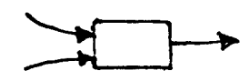
\includegraphics[scale=0.7]{figure3_block.png}}

described by a rate expression giving, $F$, the net flux carried by the block. Similarly there were `regulatory blocks' represented by, \scalebox{2}{$\diamond$} and quantitatively described by a regulatory function, $R$, giving the fraction by which the maximal activity of a structural locus should be multiplied to take account of regulation.

The concept of the sensitivity coefficient $C_{P}^{M}$ was introduced as a means to describing and measuring the nett effect of changes in genetically determined parameters on some systemic property say the measure $\olsi{M}$. Even with the simplest rate expression, a number of parameters are associated with each block and this number increases considerably when bimolecularity, regulation and inhibition has to be introduced. Insofar as all such parametric changes can affect the system only by acting through the one block, it is convenient to consider their common effect by defining a new coefficient, the `block coefficient'. It will be shown that, on the other hand, the differences between the effects of parameter within a given block are described by a set of further coefficients descriptive of the behaviour of the isolated block.

The block coefficient is introduced by the following considerations. A fairly general set of equations defining the S.S. was of the form
%
\begin{equation}
\sum \lambda_{i \mathbf{j}} F_{\mathfrak{j}}=0
\label{eqn:312}
\end{equation}
%
Where $F_{j}$ stands for a 'complete' transformational expression involving, in general, both a rate expression $f_{j}$ and a regulatory function $R_{k}$.

Consider a new `constructed' system related to the original one in that each complete transformational expression, in (3.32), is replaced by a modified form $F^{\prime}_j$ obtained by multiplying each $F$ in \eqref{eqn:312}  by an extra parameter $\alpha_{j}$. When the constructed system has all its $\alpha_{j}$ equal to unity it will, of course, have the same S.S. solution as the original system and will behave identically with regard to other parameter variations. The equations defining the S.S. of the constructed system will be
%
\begin{equation}
\sum \lambda_{ij} \alpha_{j} F_{j}=0
\label{eqn:313}
\end{equation}
%
The coefficient of a measure $\olsi{M}$ with respect to, say, the 3rd transformational block in the constructed system can now be defined in the usual way as
%
\begin{equation}
C_{\alpha_{3}}^{\olsi{M}}=\frac{\alpha_{3}}{\olsi{M}} \cdot \frac{\partial \olsi{M}}{\partial a_{3}}
\label{eqn:314}
\end{equation}
%
The block coefficient in the original system is then defined as $C^{\olsi{M}}_{\alpha_3}$ evaluated with all $\alpha$'s equal to unity, that is around the position where the original and the constructed systems behave identically.

It will now be shown how the sensitivity coefficient, $C_{P}^{\olsi{M}}$, is related to $\mathrm{C}_{\alpha_{3}}^{\olsi{M}}$ when $P$ is a parameter embedded within the expression $F_{3}$.

The relation can be discovered by considering that it is always possible to make simultaneous small changes $\Delta \alpha_{3}$ and $\Delta \mathrm{P}$ such that the S.S. solution, $\olsi{S}_{i}$, will remain completely unchanged, as also will all measures on this S.S. not directly involving $\alpha_{3}$ or $P$. This gives rise to two relations.

Considering first, the system as a whole it gives rise to the relation
%
\begin{equation}
C_{\alpha_{3}}^{\olsi{M}} \cdot \frac{\Delta \alpha_{3}}{\alpha_{3}} + C_{P}^{M} \cdot \frac{\Delta P}{P} = 0 \tag{a}
\label{eqn:315a}
\end{equation}
%
On the other hand considering the transformational flux expression, $F_{3}^{\prime}$, in isolation, and noting that the only quantities occurring in it which are subject to change are $\alpha_{3}$ and $P$ and that these produce zero net effect we have
%
\begin{equation}
\left[\mathrm{C}_{\alpha_{3}}^{\mathrm{F}_{3}^{\prime}}\right] \cdot \frac{\Delta \alpha_{3}}{\alpha_{3}} + \left[\mathrm{C}_{\mathrm{P}}^{\mathrm{F}^{\prime}_3}\right] \cdot \frac{\Delta \mathrm{P}}{\mathrm{P}}=0 \tag{b}
\label{eqn:315b}
\end{equation}
%
in (b) the square brackets are used to denote coefficients of the transformational flux expression, considered in isolation from the and rest of the system and with respect to one of its arguments.

Combining (a) and (b) and remembering that, since $\mathrm{F}_{3}^{\prime}=\alpha_{3} \cdot \mathrm{F}_{3^{\prime}}$
%
$$
\left[C^{F^{\prime}}_{\alpha_3}\right]=1 \text { and }\left[C_{P}^{F^{\prime}}\right] \equiv\left[C_{P}^{F}\right] \text { we get }
$$
%
\begin{equation}
C_{P}^{\olsi{M}} = C_{\alpha_3}^{\olsi{M}} \cdot\left[C_{P}^{F_{3}}\right]
\label{eqn:315}
\end{equation}
%
The relationship \eqref{eqn:315} which applies in both the original and the constructed system, states that the sensitivity of a measure $\olsi{M}$ to a parameter $P$ will depend jointly on the sensitivity of $\olsi{M}$ to the block in which $P$ acts and on the sensitivity of the flux through this block, when considered in isolation from the rest of the system, to the parameter $P$ itself.

In the more general case where the parameter $P$ occurs in connection with several transformational blocks (such as multiple inhibition by an external. substance) the relation \eqref{eqn:315} becomes
%
\begin{equation}
C_{P}^{\olsi{M}}=\sum C_{\alpha_{r}}^{\olsi{M}} \times \left[C_{P}^{F_r}\right]
\label{eqn:316}
\end{equation}
%
where the summation effectively extends over all blocks influenced directly by P. Consider for example a system, as indicated below, containing a group of three enzymes having rate expressions $f_{1}, f_{2}, f_{3}$ and each under co-ordinate control from a block with regulatory function $\mathrm{R_1}$

\begin{center}
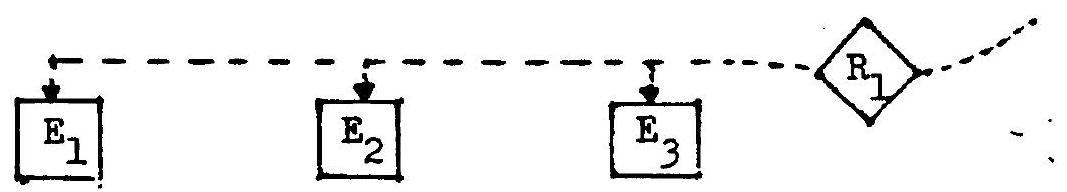
\includegraphics[max width=\textwidth]{2023_01_30_a974a42f7b7381f3f940g-101}
\end{center}

The separate $f$ flux expressions will then be $f_{1} \times R_{1}, f_{2} \times R_{1}, f_{3} \times R_{1}$, and the sensitivity of any measure $\olsi{M}$ to the regulatory block, $R_{1}$, can be considered as the sensitivity to a parameter $\beta$, of value unity, multiplying into the regulatory function $\mathrm{R}_{1} \cdot$ Using the relation \eqref{eqn:316} we get
%
$$
C_{\beta}^{\olsi{M}} = C_{\alpha_{1}}^{\olsi{M}_{1}} \cdot \left[C_{\beta}^{f_{1} \times \beta \times R_1}\right] + C_{\alpha_{2}}^{M}\left[C_{\beta}^{f_{2} \times \beta \times R_1} \right]+\cdots
$$
%
Using the formal relationship \eqref{eqn:311}  to simplify the bracketed expressions we get
%
$$
C_{\beta}^{M} = C_{\alpha_{1}}^{M} + C_{\alpha_{2}}^{M} + C_{\alpha_{3}}^{M}.
$$
%
This result shows that the sensitivity to the regulatory block is just the sum of the sensitivities to the separate transformational blocks involved in the co-ordinate regulation.

\subsection{Coefficient with respect to an enzyme}

In a system where enzyme quantities are specified as parameters, that is one in which no gene control loops are operative, all flux expressions will be of the form
%
\begin{equation}
F_{j}=E_{j} \times f_{j}(--)
\label{eqn:317}
\end{equation}
%
Using, relation \eqref{eqn:315}  to connect the block coefficient to the enzyme we have
%
$$
C_{E_j}^{M}= C_{\alpha_{j}}^{M} \cdot\left[{C_{E}^{F_j}}\right]
$$
%
then using \eqref{eqn:317} and the formal relationship \eqref{eqn:311}
%
$$
C_{E_j}^{M} = C_{\alpha_j}^{M} \left[ C_{E_j}^{E^j} \right] + \left[ C^{f_j}_{E_j}\right] = C_{\alpha_{j}}^{M}(1+0)
$$
%
so that
%
\begin{equation}
C^M_{E_j} \equiv C^M_{\alpha_j}
\label{eqn:318}
\end{equation}

Thus for such a system, the block coefficient is synonymous with the coefficient with respect to enzyme quantity previously considered in CH. 1. When, however, the enzyme level is subject to control there is no such identity since $E_{j}$ is no longer a parameter and $C_{E_{j}}^{M}$ has no clear meaning.

\subsection{Coefficient with respect to turnover number}

Even when enzyme quantity is subject to control, the rate expression will still be of the form $F_{j}=E_{j} (\cdots) t_{j} f_{j} (\cdots)$ Where the enzyme level, $E_{j}$, is now a function of some sort and $t_{j}$ is the turnover number. In this case an argument, similar to that above, will show that
%
\begin{equation}
C_{\alpha_{j}}^{M} \equiv C_{t_{j}}^{M}
\label{eqn:319}
\end{equation}
%

\subsection{Coefficient with respect to gene dosage}

When control is operative and on the assumption that the system under consideration is a small part of some larger system the gene dosage parameter $g_{j}$ introduced in the last chapter will always appear multiplied into the complete flux expression for the jth transformation or
%
$$
F_{j}=g_{j} \times t_{j} \times f_{j}(-) \times n_{jk} \times R_{k}(-)
$$
%
Therefore once again
%
\begin{equation}
\mathrm{C}_{\alpha_j}^{\olsi{M}} \equiv \mathrm{C}_{g_j}^{\olsi{M}}.
\label{eqn:320}
\end{equation}
%
A slight correction to this result will be necessary if it is conceded that the system under consideration is not a small part of a larger system but it will still be approximately true. Another difficulty arises, in relation to the meaning of $\mathrm{C}_{g_{j}}^{M}$ in (3.2.0), because in most organisms it is not possible to vary $g_{j}$ continuously. However, this problem will not arise in e.g. Neurospora where $g_{j}$ can be varied almost continuously

\section{Measurement of coefficients in a `real' system}

From the foregoing it can be seen that in understanding a real system considerable insight will be obtained if the sensitivity of a selected set of measures can be determined even with respect to each transformational block, rather than for all parameters. These block coefficients cannot usually be measured as $C_{E}^{\olsi{M}}$ since in most systems there is some degree of enzyme control and enzyme quantity is not a true parameter. However, there is no such objection to obtaining the block coefficients via $C_{t_j}^{\olsi{M}}$ or $C_{g_{j}}^{\olsi{M}}$ and both of these methods have been employed. Even so several difficulties arise in practice. Thus, since it is not easy, to measure small changes in $\olsi{M}$ and $P$ with sufficient accuracy, it will usually be necessary to measure $\olsi{M}$ as accurately as possible for a number of more widely spaced `P' values and construct a smooth curve showing the relationship between $\olsi{M}$ and $P$ when all other parameters are held constant. From this curve $C_{P}^{\olsi{M}}$ can be estimated around the original $P$ value using the definition (3.6). When the sensitivity with respect to external concentration (of type $X$) is required no further difficulties arise since such quantities can be varied continuously and measured with reasonable accuracy. However, in order to measure internal `block' coefficients it is necessary to produce a controlled change in a single internal (genetically controlled) parameter and this is not always simple, or indeed possible.

For example, one way of estimating the block coefficient of an enzyme would be to measure $C_{t}^{M}$ using a series of revertants from a mutant in which the activity of the enzyme had been abolished by a mutation at its structural locus. Unfortunately each of these `new' proteins would not only have a different turnover number from the original enzyme but, in general, also different values for all the other kinetic parameters characterising the protein. In such a case it is only possible to plot $\olsi{M}$ against turnover number after establishing that other kinetic parameters are effectively uncharged. A method of this general type has been employed by C. Chilcott (Honours Thesis, Edinburgh, 1961) and B. I. Barthelmess (personal communication) using revertants in the arginine pathway of N.crassa. Another method, which is intended to avoid the complication of simultaneous changes occurring in several parameters, is to attempt to alter only the quantity of a particular structural gene. In principle this can be done by altering the `dose', that is the parameter $g_{j \text { ' }}$ and estimating the block coefficient via $\mathrm{C}_{\mathrm{g}_{j}}^{\mathrm{M}}$.

A way in which a particular $g_{j}$ can be altered almost continuously without altering anything else is by constructing heterokaryons in fungi between wild type and a strain in which activity at the structural locus in question is abolished. By varying the input of the two types contributing to the heterokaryon the dosage of the structural gene in question can be controlled over a considerable range. A method of this general type has been employed by W. Tateson (Ph.D. Thesis, Edinburgh, 1971), also for steps in the arginine pathway of Neurospora.

Since it is clear that the determination of coefficients by these `direct' experiments is extremely laborious, it is important, to establish any further general properties of coefficients, particularly in relation to the expected distribution of control between different blocks and to any 'diagnostics' which would make it easier to determine the pattern of coefficients experimentally. We will return to this subject after considering the various relations between coefficients and demonstrating how the coefficient values arise from measurable properties of the individual transformation blocks.

\section{Summation properties of block coefficients}

At the end of CH.I it was shown, relation (1.31), that the sum of the flux-control coefficients in a chain of non linear enzymes was equal to unity. Now that we have suitably extended the definition of
coefficient to general networks and networks in which enzyme quantities cannot be treated as a parameter it will be demonstrated that this and other properties still hold, being indeed a very general and simple consequence of the block structure of metabolic systems.

Thus consider the general S.S. equations (3.13) defining the constructed system:

$$
\sum \lambda_{ij} \alpha_j F_j = 0
$$

I. ``The sum of the sensitivity coefficients of any given pool, $S$, with respect to each of the separate transformation blocks in the system is zero''

\tcbset{colback=yellow!10!white, colframe=red!50!black,leftrule=0.45mm,
        highlight math style= {enhanced, %<-- needed for the ’remember’ options
            colframe=red,colback=red!10!white,boxsep=0pt}
        }

\begin{tcolorbox}[ams equation]
\sum_{j=1, \ldots m} C_{\alpha_j}^{\olsi{S}}=0
\label{eqn:321}
\end{tcolorbox}


II. ``The sum of the sensitivity coefficients of any given flux, $F$, in the system with respect to each of the separate transformation blocks in the system is unity''

\begin{tcolorbox}[ams equation]
\sum_{j=1, \ldots m} C_{\alpha_j}^{\olsi{F}} = 1
\label{eqn:322}
\end{tcolorbox}

These two results can be obtained by supposing that the same fractional differential change $x$ is made in all the $\alpha_{j}$. Then for a given pool the fractional response is found by summing up the responses predicted from the separate sensitivities or:
%
$$
\frac{\Delta S}{S}= \sum C_{\alpha_{j}}^{S} \cdot x
$$
%
But $\frac{\Delta S}{S}=0$, from the co-ordinate property. Therefore $\sum \mathrm{C}_{\alpha_{j}}^{\mathrm{S}}=0$, as required.

In the case of the flux coefficients we have, similarly.

$$
\frac{\Delta F}{F} = \sum C_{\alpha_{j}}^{F} \cdot x
$$
%
and in this case the co-ordinate property predicts $\frac{\Delta \mathrm{F}}{F}=\mathrm{x}$, so that
%
$$
x = \sum \mathrm{C}_{\alpha_{\mathbf{j}}}^{F} \cdot x \text { or } \sum \mathrm{C}_{\alpha_{\mathbf{j}}}^{F}=1 \text {, as required }
$$
%
The result (3.22) is particularly useful in relation to the problem of discovering the rate-controlling enzyme for a particular flux in an experimental situation. Thus it predicts that provided that, the structure is such that all coefficients are +ve, the value of the coefficient for a rate controlling enzyme would have to be close to unity. This means that a single experiment on a suspected enzyme can confirm or deny the hypothesis that it is the rate controlling one. Whereas in the absence of an expected value for the coefficient of a rate-controlling enzyme it would be necessary to perform such an experiment for all the enzymes in the system and compare their values, which is hardly practical.. Unfortunately no simple prediction can be made when -ve coefficients are a possibility, as for example in systems having divided pathways.

The result (3.21) for pool coefficients shows that they must be both +ve and -ve but otherwise places no limit on their values. In a later section it will be shown, by algebraic study of a simples system, that there is no general restriction on the values which can be taken by the individual coefficients of either pools or fluxes.

\section{Elasticities of complete flux expressions}

In the preceding discussion of block coefficients the sensitivity of a complete flux expression, $F_{j}$, in isolation from the rest of the system was used, that is for one of its arguments when all others are held at their S.S. levels. This was expressed by enclosing the ordinary sensitivity coefficient notation in square brackets as for example $\left[C_{P}^{F_r}\right]$ in (3.16). Such terms occur frequently in relations between system block coefficients and it is useful to distinguish them from these by a suitable notation. Accordingly we call them `elasticities' writing the above example as $\varepsilon_{p}^{F_r}$.
%
\begin{equation}
C_{P}^{\olsi{M}} = \sum C_{\alpha_{r}}^{\olsi{M}} \cdot \varepsilon^{F_r}_P
\label{eqn:323}
\end{equation}
%
The elasticities of a flux expression are, of course, not constant but will depend on the operating conditions of the appropriate enzymes under in vivo S.S. conditions. In principle they could be measured by extracting the appropriate enzymes, reconstructing their exact operating conditions in vitro and determining the sensitivity of the flux to separate modulations in substrates, products, regulators etc. In practice such a procedure is not usually feasible but it will be shown later in this chapter that it is still possible to obtain estimates of all elasticities by considering data from modulation experiments carried out around an existing S.S. in vivo.

Using the idea of elasticity it becomes straightforward to write down the response of a typical flux expression, considered in isolation, to variation in it's arguments. Thus consider the subunits indicated below which together define the flux expression $F_{1}$

\begin{center}
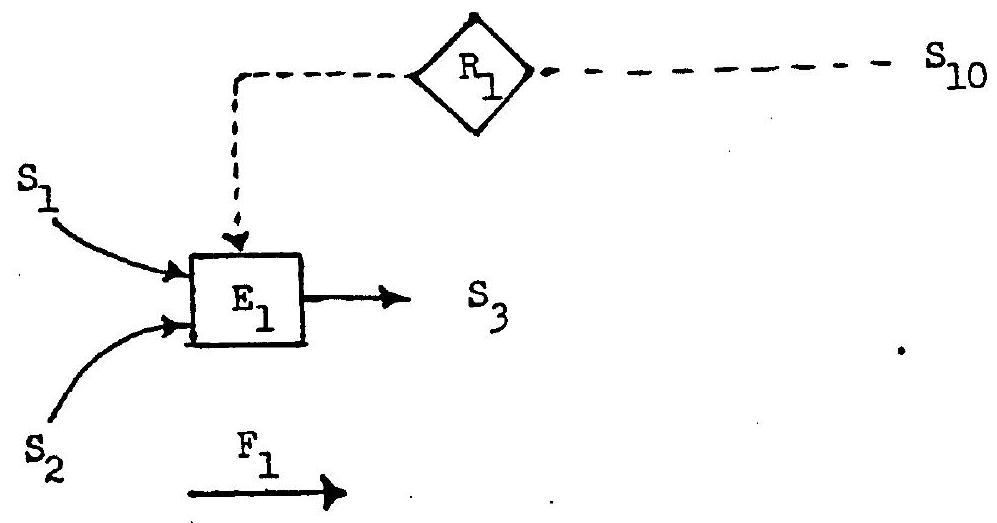
\includegraphics[max width=0.6\textwidth]{2023_01_30_a974a42f7b7381f3f940g-110}
\end{center}

If $\alpha_{1}$ is modulated it will produce consequent changes in $S_{1}, S_{2}, F_{1}$ and throughout the system, but it will. always be true that:
%
$$
\frac{\Delta F_{1}}{F_{1}} = \varepsilon^{F_1}_{\alpha_{1}} \cdot \frac{\Delta \alpha_{1}}{\alpha_{1}} + \varepsilon^{F_{1}}_{S_{1}} \cdot \frac{\Delta S_{1}}{S_{1}} + \varepsilon_{S_{2}}^{F_{1}} \cdot \frac{\Delta S_{2}}{S_{2}} + \ldots
$$
%
Here the complete flux expression $F_{1}$ involves more than just the rate equation, being of the form:
%
$$
F_{1}=\alpha_{1} \cdot f_{1}\left(S_{1}, S_{2}, S_{3}\right) \cdot R\left(S_{10}\right)
$$
%
Consequently the elasticities can be simplified, for example
%
$$
\varepsilon_{\alpha_{1}}^{F_{1}} = 1
$$
%
$$
\varepsilon_{S_{1}}^{F_{1}} = \varepsilon_{S_{1}}^{f_{1}}
$$
%
and $\quad \varepsilon_{S_{10}}^{F_{1}}=\quad \varepsilon^{R_{1}}_{S_{10}}$. So that
%
$$
\frac{\Delta F_{1}}{F_{1}}=\frac{\Delta \alpha_{1}}{a_{1}}+ \varepsilon_{S_{1}}^{f_{1}} \cdot \frac{\Delta S_{1}}{S_{1}} + \varepsilon_{S_{2}}^{f_{1}} \cdot \frac{\Delta S_{2}}{S_{2}}+ \varepsilon_{S_{3}}^{f_2} \cdot \frac{\Delta S_{3}}{S_{2}}+ \varepsilon_{S_{10}}^{R} \frac{\Delta S_{10}}{S_{10}}
$$

Expressions of this type will be used in subsequent discussion.

\section{Relative Importance of two successive enzymes in a straight chain}

The situation often arises, even within a complex system, that two enzymes can be found such that the product of one is the substrate of the next and has no strong interaction with any other protein in the system. Such a situation is indicate below for two hypothetical enzymes, $\mathrm{E}_{1}$ and $E_{2}$, which may be quite complicated such as being bimolecular and suffering inhibition.

\begin{center}
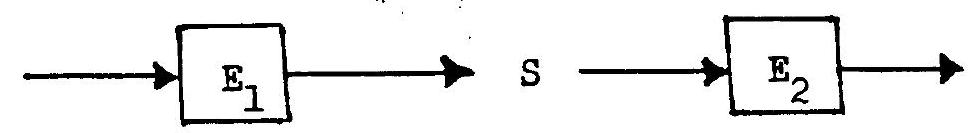
\includegraphics[max width=0.6\textwidth]{2023_01_30_a974a42f7b7381f3f940g-112}
\end{center}

Provided that $S$ only affects $E_{1}$ and $E_{2}$ it will always be possible to make simultaneous changes in the block parameters $\alpha_{1}, \alpha_{2}$ such that only $S$ is altered. This is achieved by increasing $\alpha_{1}$ and then decreasing $\alpha_{2}$ so as to exactly cancel the effect on all pools and fluxes other than the common pool S. Suppose that such an operation produces a small fractional change $\frac{\Delta S}{S}$ in S. Considering the flux expression, $F_{1}$, in isolation from the rest of the system and noting that simultaneous changes in $\alpha_{1}$ and $S$ produce no change in $F_{1}$, we have, using the elasticity notation
%
$$
\varepsilon_{\alpha_{1}}^{F_{1}} \cdot \frac{\Delta{ }^{\alpha_1}}{\alpha_1} + \varepsilon_S^{F_1} \cdot \frac{\Delta \mathrm{S}}{\mathrm{S}}=0
$$
%
or
%
\begin{equation}
\quad \frac{\Delta \alpha_{1}}{\alpha_{1}} = -\varepsilon_{S}^{F_1} \cdot \frac{\Delta S}{S} \tag{a}
\label{eqn:323a}
\end{equation}
%
Similarly for $E_2$
\begin{equation}
\frac{\Delta \alpha_2}{\alpha_2}=-\varepsilon_S^{F_2} \cdot \frac{\Delta S}{S} \tag{b}
\label{eqn:323b}
\end{equation}

Finally, since the simultaneous changes in $\alpha_{1}, \alpha_{2}$ have no effect on any system measure, except $S$, we have for the whole system,
%
\begin{equation}
C_{\alpha_{1}}^{M} \cdot \frac{\Delta \alpha_{1}}{\alpha_{1}}+C_{\alpha_{2}}^{M} \cdot \frac{\Delta \alpha_{2}}{a_{2}}=0 \tag{c}
\label{eqn:323c}
\end{equation}
%
where $C_{\alpha}^{M}$ are the ordinary systemic block coefficients of a measure M.

Combining the three equations $a, b, c$, we have that for two successive enzymes in a chain the ratio of their sensitivity coefficients $C_{1}, C_{2}$ for any measure is given by

\begin{tcolorbox}[ams equation]
\frac{C_1}{C_2} = -\frac{\varepsilon^{F_2}_2}{\varepsilon^{F_1}_1}
\label{eqn:324}
\end{tcolorbox}

This result will be true no matter how complex the system within which the two enzymes are embedded.

For example consider two `linear' enzymes, $E_{1}$ and $E_{2}$ within some larger system as indicated below and suppose them subject to repression via a manression function $R$ and the first one to non competitive inhibition with an inhibitory function $\phi$.

\begin{center}
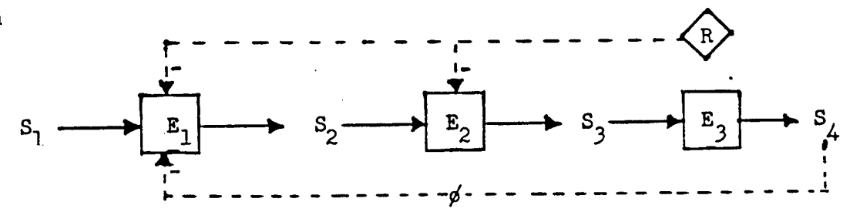
\includegraphics[max width=\textwidth]{figure3_324.png}
\end{center}

To find the relative importance of their block coefficients for a.1 measures (other than $S_2$) we apply $\left(3.24\right)$ or
%
$$ \frac{C_1}{C_2} = -\frac{\varepsilon_{S_2}^{F_2}}{\varepsilon_{S_2}^{F_1}} = -\frac{\varepsilon_{S_2}^{\left(\alpha_2 \cdot f_2 \cdot R\right)}}{\varepsilon_{S_2}^{\left(\alpha_1 \cdot f_1 \cdot R \cdot \phi\right)}} $$
%
Using the formal relation (3.11) to simplify this we get
%
$$
\frac{C_{1}}{C_{2}}=\frac{\varepsilon_{S_{2}}^{\alpha_{2}}+\varepsilon_{S_{2}}^{f_{2}}+\varepsilon_{S_{2}}^{R}}{\varepsilon_{S_{2}}^{a_{1}}+\varepsilon_{S_{2}}^{f_{1}}+\varepsilon_{S_{2}}^{R}+\varepsilon^\phi_{S_{2}}} = \frac{0+\varepsilon_{S_{2}}^{f_{2}}+0}{0+\varepsilon_{S_{2}}^{f_{1}}+0+0}
$$
%
or
%
$$\quad \frac{C_{1}}{C_{2}}=\frac{\varepsilon_{S_{2}}^{f_{2}}}{\varepsilon_{S_{1}}^{f_{2}}}$$
%
so that the ratio of block coefficients depends on the ratio of the elasticities of the two rate expressions with respect to the common pool. In particular, if the reactions are linear, $f_{1}$ will be of the form
%
$$ f_{1}= v_{1}\left(S_{1}-\frac{S_{2}}{K_{1}}\right)$$,
%
and using the definition (3.3) for the coefficient we have
%
$$
\varepsilon_\mathrm{S_2}^{f_1} = \left[\mathrm{C}^{\mathrm{f}_{1}}_{\mathrm{S}_{2}}\right] = \mathrm{S_2} \frac{\partial\left(\log \mathrm{f}_{1}\right)}{d\mathrm{S}_{2}}=\frac{\mathrm{S}_{2} / \mathrm{K}_{1}}{\mathrm{S}_{1}-\mathrm{S}_{2} / \mathrm{K}_{1}}
$$
%
$$
\begin{aligned}
& \text { similarly } \quad \varepsilon^{f_2}_{S_2} = \frac{\mathrm{S}_{2}}{\mathrm{S}_{2} - \mathrm{S}_{3} / \mathrm{K}_{2}} \\[5pt]
& \text { so that } \quad \frac{\mathrm{C}_{1}}{\mathrm{C}_{2}}=\frac{\left(\mathrm{S}_{1}-\mathrm{S}_{2} / \mathrm{K}_{1}\right)}{\left(\mathrm{S}_{2}-\mathrm{S}_{3} / \mathrm{K}_{2}\right)} \cdot \mathrm{K}_{1}
\end{aligned}
$$
%
The two terms in numerator and denominator will be recognised as the `out-of-equilibrium' of the two steps. This confirms and extends the result in CH.I concerning the usefulness of the `out-of-equilibrium' term as a diagnostic for rate control in simple cases.

\section{Relation between the coefficients of all blocks affected a given pool}

The relation (3.24) applying to two successive blocks affected by a common pool can now be generalised to cases where the given pool influences more than two enzymes, as for example if it is a signal for repression or perhaps at the dividing point of a branched pathway.

Since it turns out that the argument does not depend on the \underline{flux} relationship of the influenced enzymes it will be sufficient to refer to a general pool influence diagram, indicated below for enzymes $\mathrm{E}_{1}, \mathrm{E}_{2}, \mathrm{E}_{3}$ and $E_{4}$ which are all affected by pool S. In this diagram the dotted lines signify influence, that is non zero elasticities with respect to $S$, and flux arrows, which may coincide, have been omitted.

\begin{center}
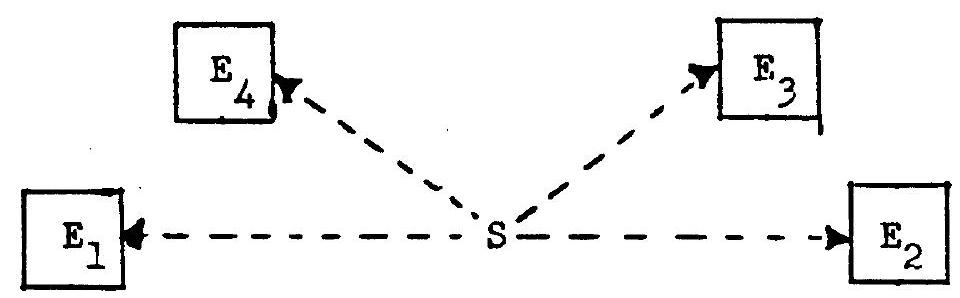
\includegraphics[max width=0.8\textwidth]{2023_01_30_a974a42f7b7381f3f940g-115}
\end{center}

As in the previous argument, when S affected only two enzymes, it is always possible to make simultaneous movements in $\alpha_{1}, \alpha_{2}, \alpha_{3}$ and $\alpha_{4}$ such that only $S$ is changed, all other pools in the system remaining constant. By considering $F_{1}$ in isolation we must have:
%
$$ 0 = \frac{\Delta F_1}{F_1} = \varepsilon_{\alpha_1}^{F_1} \cdot \frac{\Delta \alpha_1}{\alpha_1}+ \varepsilon^{F_1}_S \cdot \frac{\Delta_S}{S} $$
%
or
%
\begin{equation}
\frac{\Delta \alpha_{1}}{\alpha_{1}}=\varepsilon_{S}^{F_1} \cdot \frac{\Delta S}{S} \tag{a}
\label{eqn:324a}
\end{equation}
%
and similar relationships for $\mathrm{E}_{2}, \mathrm{E}_{3}$ and $\mathrm{E}_{4}$

Also since no measure, other than $S$, is affected by these simultaneous changes in the a values, we can write for the system as a whole
%
\begin{equation}
C_{\alpha_{1}}^{M} \cdot \frac{\Delta \alpha_{1}}{\alpha_{1}}+ C_{\alpha_{2}}^{M} \cdot \frac{\Delta \alpha_{2}}{\alpha_{2}} + \ldots =0 \tag{b}
\label{eqn:324b}
\end{equation}
%
Combining (b) with the four relationships of type (a) the connection between the system coefficients of the four blocks and their elasticities with respect to the chosen pool, $S$, is found to be:
%
\begin{equation}
C_{\alpha_{1}}^{M} \cdot \varepsilon_{S}^{F_{1}}+ C_{\alpha_{2}}^{M} \cdot \varepsilon_{S}^{F_{2}}+ C_{\alpha_{3}}^{M} \cdot \varepsilon_{S}^{F_{3}}+ C_{\alpha_{4}}^{M} \cdot \varepsilon_{S}^{F_{4}}=0
\label{eqn:325}
\end{equation}
%
This is the required generalisation of (3.24), when only two pools were involved, and clearly such an equation can be written down for every pool in the system. The relationship for each pool, of course, involves only those blocks having non-zero elasticities with respect to it. Expressed generally the relationship is:
%
\begin{equation}
\sum C_{\alpha_{j}}^{M} \cdot \varepsilon_{S}^{j}=0
\label{eqn:326}
\end{equation}
%
Where $\varepsilon_{S}^{j}$ is short for $\varepsilon_{S}^{F_j}$.

For a system containing $n$ pools there will be a relations of type (3.26) and within each of these most of the $\varepsilon_{S}^{j}$ will be zero, since most pools influence only a few enzymes. A special case arises in the above arguments when the pool being modulated is \underline{itself} taken as the measure. When this is so the result (3.26) will be slightly modified. Thus the relationship (b), above, now becomes
%
$$
C_{\alpha_{1}}^{S} \cdot \frac{\Delta \alpha_{1}}{\alpha_{1}} + C_{\alpha_{2}}^{S} \cdot \frac{\Delta \alpha_{2}}{\alpha_{2}} + \cdots \cdot=\frac{\Delta S}{S}
$$
%
and when combined with (a) and written in the `elasticity' notation yields
%
$$
\sum C_{\alpha_{j}}^{S} \cdot \varepsilon_{S}^{j} = -1
$$
%
This can be generalised for the case where the measure is any pool $S_{i}$ and the modulation is performed on any pool $\mathrm{S}_{\mathrm{k}}$, when
%
\begin{equation}
\sum C_{\alpha_{j}}^{S_{i}} \cdot \varepsilon_{S_{k}}^{j}=-\delta_{k}^{i}
\label{eqn:327}
\end{equation}
%
In relation (3.27), $\delta_{k}^{i}=1$ when $i=k$ and zero when $i \neq k$

Clearly in an $n$ pool $m$ block system it will be possible to write down $n$ relations of type (3.26) or (3.27) connecting the m block coefficients of any given measure. However, since for a general system $m \geq n+1$, these will not suffice to determine the separate block coefficients and it will be necessary to write down a further $(m-n)$ relations between the block coefficients.

\section{System coefficients and a given independent flux}

{\bf Relations between system coefficients for all blocks contributing to a given independent flux}

The $(m-n)$ supplementary relationship referred to above can be written down by considering the different distinct ways in which it is possible to modulate various $\alpha_{j}$ and change the relative fluxes in the S.S. condition of the network without altering any pools. Once this has been achieved it will be possible to solve the block coefficients in terms of the underlying elasticities.

In general this can be done in exactly $(m-n)$ distinct ways, each one corresponding to that set of a modulations which alters a particular one of the $(m-n)$ independent fluxes without affecting any of the other independent fluxes or any of the pools. Thus a local flux can be expressed as a linear combination of the independent fluxes, as in the example previously given on p.53 CH.II.

For the jth dependent flux,

\begin{equation}
F_{j}= \sum a_{jk} Y_{k}
\label{eqn:328}
\end{equation}

Where $Y_{k}$ stands for the values of the designated set of independent fluxes at the S.S. and the $a_{jk}$ can be found from the stoichiometric matrix $\left[\lambda_{ij}\right]$ Suppose that we wish to find the set of `$\alpha$ ' modulation which will affect the independent flux $Y_{1}$ and no other independent flux or pool. Clearly if, by differentiation of the stoichiometric relation (3.28), $\frac{\Delta Y_{1}}{Y_{1}}$ is the small fractional change in one of the independent fluxes, $Y_{1}$, then the charge in a local flux, $F_{j}^{\prime}$, of the constructed system must be given by
%
\begin{equation}
\frac{\Delta F_{j}^{\prime}}{F_{j}^{\prime}} = \left[\frac{Y_{1}}{F_{j}^{\prime}} \cdot \frac{\partial\left(\sum \alpha_{jk} Y_{k}\right)}{\partial Y_{1}}\right] \cdot \frac{\Delta Y_{1}}{Y_{1}}
\label{eqn:329}
\end{equation}
%
a convenient notation for this is
%
\begin{equation}
\frac{\Delta F_{j}^{\prime}}{F_{j}^{\prime}} = \varepsilon_{Y_{1}}^{F^\prime_j} \cdot \frac{\Delta Y_{1}}{Y_{1}}
\label{eqn:330}
\end{equation}
%
In relation (3.30) $\varepsilon^{F^\prime_j}_{Y_1}$ stands for what may be called the `stochiometric elasticity' of $F_{j}^{\prime}$ with respect to the independent flux $Y_{1}$. Carrying out the differentiation of $(3.28)$ we have
%
$$
\varepsilon_\mathrm{Y_1}^{F^\prime} = \frac{a_{j1} Y_{1}}{\sum a_{jk} {Y}_{k}}
$$
%
and it appears that the stoichiometric elasticity measures the ``proportion of the jth flux which is accounted for by a given independent flux''. If now at each transformational block the $\alpha_{j}$ is changed proportionally to the stoichiometric elasticity with respect to the independent flux $Y_{1}$, the final result will be that the necessary flux changes are achieved without altering any pools and without altering any independent fluxes other than $Y_{1}$. Since for any pool. S the set of a modulations just described has no effect we have
%
$$
\sum C_{\alpha_{j}}^{S} \cdot \frac{\Delta \alpha_{j}}{\alpha_{j}}=0 \text {, where all the. } \alpha_{j} \text { are equal to } \varepsilon_{Y_{1}}^{F_{j}^{\prime}} \cdot \frac{\Delta Y_{1}}{Y_{1}}
$$
%
so that
%
\begin{equation}
\sum C_{\alpha_{j}}^{S} \cdot \varepsilon_{Y_1}^{F_{1}^{\prime}} = 0
\label{eqn:331}
\end{equation}
%
Relations of the type (3.31) provide the necessary $(m-n)$ equations referred to earlier since there is one such relation for each of $(m-n)$ independent fluxes. If the measure involved is the independent flux itself then
%
$$
\sum C_{\alpha_{j}}^{Y_{1}} \cdot \frac{\Delta \alpha_{j}}{\alpha_{j}}=\frac{\Delta Y_{1}}{Y_{1}} \text {, where } \frac{\Delta \alpha_{j}}{\alpha_{j}}=\varepsilon_{Y_{1}}^{F_{j}^{\prime}} \cdot \frac{\Delta Y_{1}}{Y_{1}}
$$
%
so that
%
\begin{equation}
\sum C_{\alpha_{j}}^{Y_{1}} \cdot \varepsilon_{Y_{1}}^{F_{j}^{\prime}}=1
\label{eqn:332}
\end{equation}
%
or more generally
%
\begin{equation}
\sum C_{\alpha_{j}}^{Y_{i}} \cdot \varepsilon_{Y_{k}}^{F_{j}^{\prime}}=\delta_{k}^{i}
\label{eqn:333}
\end{equation}
%
The (m-n) relation of type (3.31) or (3.33) obtained by considering modulation of the different independent fluxes and involving the appropriate `stochiometric elasticities' are clearly similar to the $n$ relation of type (3.26) or (3.27) obtained by considering modulation of pools and involving flux expression elasticities. Together they are sufficient to determine the block sensitivities for any specified measure. The use of this will be shown in the examples which will follow.

\section{Relations between the system coefficients}

{\bf Relations between the system coefficients of different measures connected with a given block}

The relation of $(3.26),(3.27)$ and (3.31), (3.33) all connect the coefficient of a given measure with respect to different blocks. A similar type of argument can be used to establish the relationship  between the coefficient of different measures with respect to a single block so that once we have established, say, the flux coefficients $C_{\alpha_{j}}^{F}$ it will be possible to calculate from them the various pool measures $C_{\alpha_{j}}^{S}$.

Consider for example the kth block and suppose it to be influenced by $\mathrm{S}_{1}, \mathrm{S}_{2}, \mathrm{S}_{3}, \mathrm{S}_{4}$ as shown below.

\begin{center}
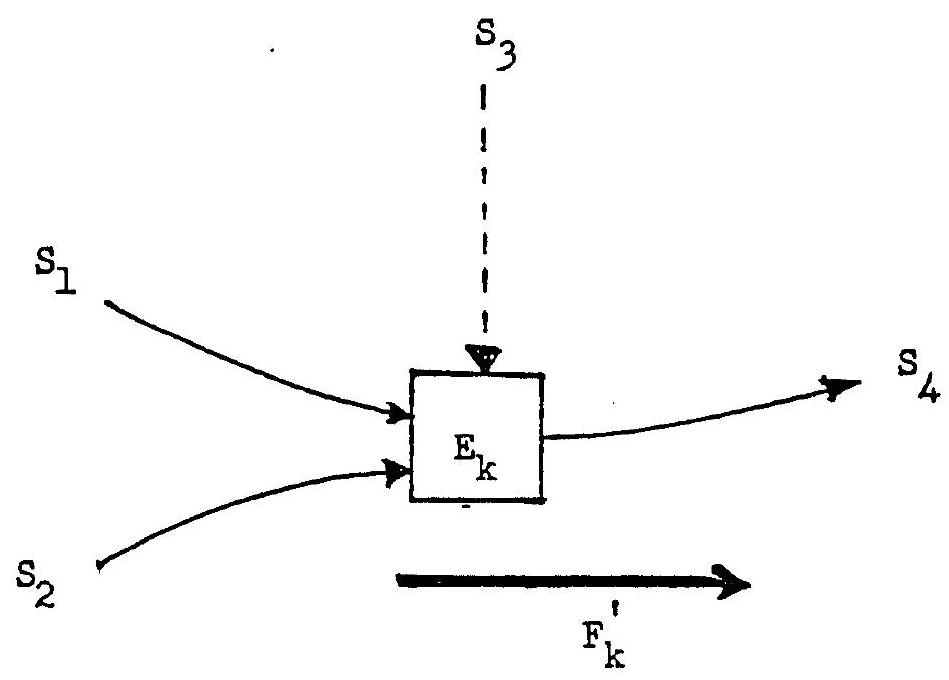
\includegraphics[max width=0.6\textwidth]{2023_01_30_a974a42f7b7381f3f940g-121}
\end{center}

Suppose that the $\alpha$ of the $j$th block is modulated by $\frac{\Delta \alpha_{j}}{\alpha_{j}}$, then considering the whole system.
%
\begin{equation}
\frac{\Delta F_{k}^{\prime}}{F_{k}^{\prime}}= C_{\alpha_{j}}^{F_{k}^{\prime}} \cdot \frac{\Delta \alpha_{j}}{\alpha_{j}}, \frac{\Delta S_{1}}{S_{1}}=C_{\alpha_{j}}^{S_{1}} \cdot \frac{\Delta \alpha_{j}}{\alpha_{j}}, \ldots \text { etc. }
\label{eqn:334}
\end{equation}
%
Considering now the kth block in isolation we can write 99.
%
$$
\begin{aligned}
& \frac{\Delta F_{k}^{\prime}}{F_{k}^{\prime}}= \varepsilon_{\alpha_{j}}^{F_{k}^{\prime}} \cdot \frac{\Delta \alpha_{j}}{\alpha_{j}} + \varepsilon_{S_{1}}^{F_{k}^{\prime}} \frac{\Delta S_{1}}{S_{1}} + \varepsilon_{S_{2}}^{F_{k}^{\prime}} \cdot \frac{\Delta S_{2}}{S_{2}}+\ldots \\
& \text { Replacing the fractional changes by means of relations (3.34) this becomes } \\
& C_{\alpha_{j}}^{F_{k}^{\prime}} \cdot \frac{\Delta \alpha_{j}}{\alpha_{j}}=\varepsilon_{\alpha_{j}}^{F_{k}^{\prime}} \frac{\Delta \alpha_{j}}{\alpha_{j}}+ \varepsilon_{S_{1}}^{F_{k}^{\prime}} \cdot C_{\alpha_{j}}^{S_{1}} \cdot \frac{\Delta \alpha_{j}}{\alpha_{j}}+\ldots \\
& \text { Now } \varepsilon_{\alpha_{j}}^{F_{k}^{\prime}}=\delta_{j}^{k}, \frac{\Delta \alpha_{j}}{\alpha_{j}} \text { will cancel out and if we suppose, for example, } \\
& \text { that } C_{\alpha_{j}}^{S_{4}} \text { is unknown and the other coefficients are known we get: } \\
\end{aligned}
$$
%
\begin{equation}
C_{\alpha_{j}}^{S}=\left(C_{\alpha_{j}}^{F_{k}^{\prime}}-\delta_{j}^{k}- C_{\alpha_{j}}^{S_{1}} \cdot \varepsilon_{1}^{k}- C_{\alpha_{j}}^{S_{2}}: \varepsilon_{2}^{k}- C_{\alpha_{j}}^{S_{3}} \cdot \varepsilon_{3}^{k}\right) / \varepsilon_{4}^{k}
\label{eqn:335}
\end{equation}
%
Relations of type (3.35) and those discussed earlier can be used to progressively discover the sensitivity of measures from the known sensitivity of other measures and in many simple networks it is possible to obtain a complete sensitivity matrix in this way using only the known or estimated values of flux elasticities at the existing S.S.

\section{Application of theorems relating system coefficients to elasticities}

Some examples will now be given to make clear how sensitivity matrices may be computed from elasticities.

{\bf\large EXAMPLE I: Straight Chain with Multiple Inhibitory Loops}

Consider the straight chain system indicated below where values of elasticities around the S.S. working conditions of the transformation blocks are written inside brackets at the appropriate points in the diagram. Thus:

\begin{center}
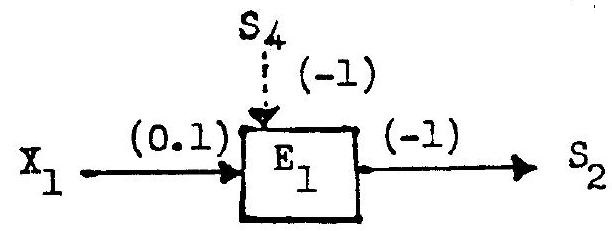
\includegraphics[max width=0.5\textwidth]{2023_01_30_a974a42f7b7381f3f940g-123}
\end{center}

means that the elasticities of enzyme 1 are: $0.1,-1,-1$, with respect to substances $\mathrm{X}_{1}, \mathrm{S}_{2}$ and $\mathrm{S}_{4}$ respectively. The negative values reflect the 'normal' behaviour that a product inhibits the forward reaction and that $S_{4}$ is a true inhibitor. The example includes three inhibitory loops, two of which are intersecting, to demonstrate how this affects the computation. Most of the elasticities have been taken as either $+1$ or -1, so that the arithmetic shall remain simple. Although quite feasible they are not intended to represent any real system.

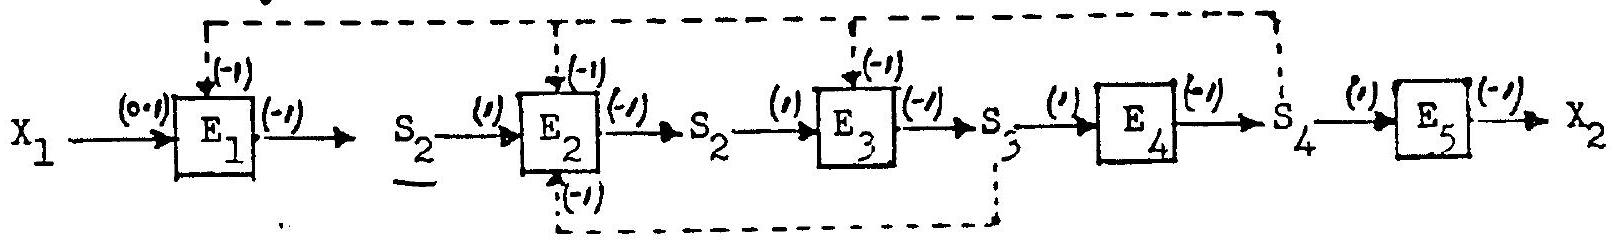
\includegraphics[max width=\textwidth, center]{2023_01_30_a974a42f7b7381f3f940g-123(1)}

The computation of a sensitivity matrix for the pools and for the pathway flux,$\left[\begin{array}{c} C^{F, S_{i}}_{\alpha_j}\end{array}\right]$ proceeds as follows:

Assume $C_{\alpha_{1}}^{F}$ to be scaled to unity, then using relations of type (3.26) arising from the virtual modulation of pools we get 101.

from pool $S_{1}: \quad C_{2}=-C_{1} \times \frac{\varepsilon_{1}^{1}}{\varepsilon_{1}^{2}}$, where $\varepsilon_{1}^{1}$ stands for $\varepsilon_{1}^{F_{1}^{\prime}}$ and so on

or

$C_{2} = -(1) \times \frac{(-1)}{(1)}=1$

from pool $S_{2}: \quad C_{3}=-C_{2} \times \frac{\varepsilon_{2}^{2}}{\varepsilon_{2}^{3}}=1$

$$S_{3}: \quad C_{4} = -\frac{\left(\varepsilon^{2}_3 \cdot C_{2} + \varepsilon^{3}_3 \cdot C_{3}\right)}{\varepsilon^{4}_3} = C_{2}+ C_{3}=2$$

$$S_{4}: \quad C_{5} = -\frac{\left(\varepsilon_{4}^{1} C_{1}+\varepsilon_{4}^{2} C_{2}+ \varepsilon_{4}^{3} C_{3}+\varepsilon_{4}^{4} \cdot C_{4}\right)}{\varepsilon_{4}^{5}}$$

$$C_{5}=C_{1}+C_{2}+C_{3} + C_{4} = 5$$

The actual coefficients must satisfy the summation theorem (3.21) and can be found by normalising the numbers just discovered, which are proportional to the flux coefficients.

This gives
%
$$
\left[C_{1}, C_{2}, C_{3}, C_{4}, C_{5}\right]=[0.1, 0.1, 0.1, 0.2, 0.5]
$$
%
Having discovered the vector of flux coefficients with respect to the different blocks $C_{\alpha_{j}}^{F}$, we may use it to successively generate the vectors for pool coefficients in the order
%
$$ C_{\alpha_{j}}^{S_4}, C_{\alpha_{j}}^{S_{3}}, C_{\alpha_{j}}^{S_{2}}, C_{\alpha_{j}}^{S_{1}} \text { using relations of type (3.35) }
$$
%
arising from the consideration of the enzymes $\mathrm{E}_{5}, \mathrm{E}_{4}, \mathrm{E}_{3}, \mathrm{E}_{2}$ in isolation.

Thus for $E_{5}$ we get: $C_{\alpha_{j}}^{S_4}=\left(C_{\alpha_{j}}^{F}-\delta_{j}^{5}\right) / \varepsilon_{4}^{5}$

$\text{which generates the vector } C_{\alpha_j}^{S_4}=[0.1, 0.1, 0.1, 0.2, -0.5]$
%

For enzyme $E_{4}$ : $
C_{\alpha_{j}}^{S_{3}}=\left(C_{\alpha_{j}}^{F}-\delta_{j}^{4}-C_{\alpha_{j}^{4}}^{S} \cdot \varepsilon_{4}^{4}\right) / \varepsilon_{3}^{4}
$

generating $ C_{\alpha_{j}}^{S_{3}}=[0.2, 0.2, 0.2, -0.6, 0] $

For enzyme $E_{3}: \quad C_{\alpha_{j}}^{S_{2}}=\left(C_{\alpha_{j}}^{F}-\delta_{j}^{3}-C_{\alpha_{j}}^{S_{3}} \cdot \varepsilon_{3}^{3}-C_{\alpha_{j}}^{S^{4}} \cdot \varepsilon_{4}^{3}\right) / \varepsilon_{2}^{3}$

generating $ C_{\alpha_{j}}^{S_{2}}=[0.4, 0.4, -0.6, -0.2, 0] $

Finally using the relationship for either $E_{1}$ or $E_{2}$, which will yield

identical results, we get $C_{\alpha_{j}}^{S_{1}}=[0.8, -0.2, -0.2, -0.4, 0.]$

The general sequence of computation can be summarised as:

\begin{center}
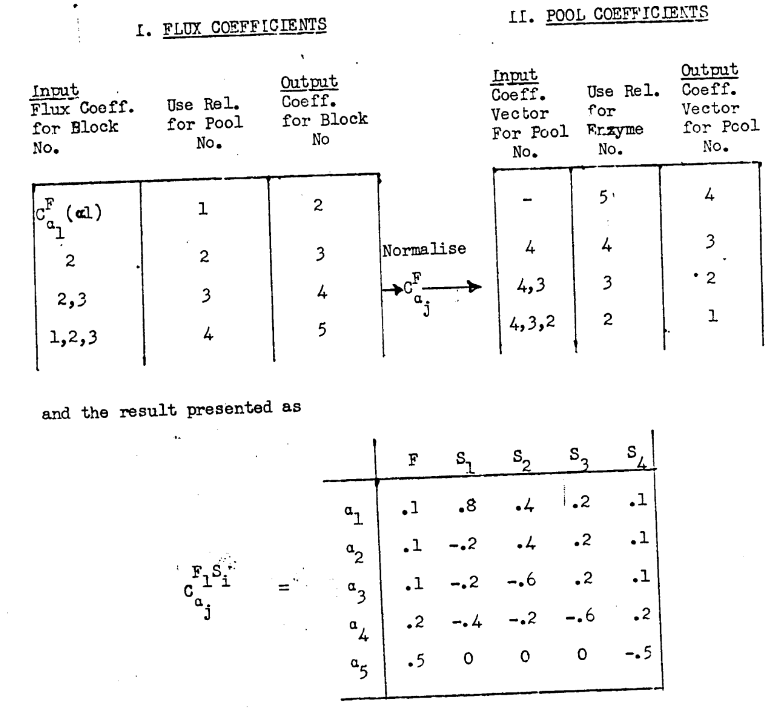
\includegraphics[max width=\textwidth]{figure3_ExampI.PNG}
\end{center}

Inspection of this matrix shows that various qualitative expectations are fulfilled. Thus a given pool always has positive coefficients for enzymes upstream from it and -ve coefficients for enzymes downstream. Furthermore all flux coefficients are +ve, as would be expected in a straight chain without positive feedback.

Two further examples follow, using the same format. These are intended to illustrate how quite complex networks can be dealt with and also to give some idea of the numerical range and the general pattern which sensitivity coefficient may take.

{\bf\large EXAMPLE II: Bimolecularly Coupled Pathways}

\begin{center}
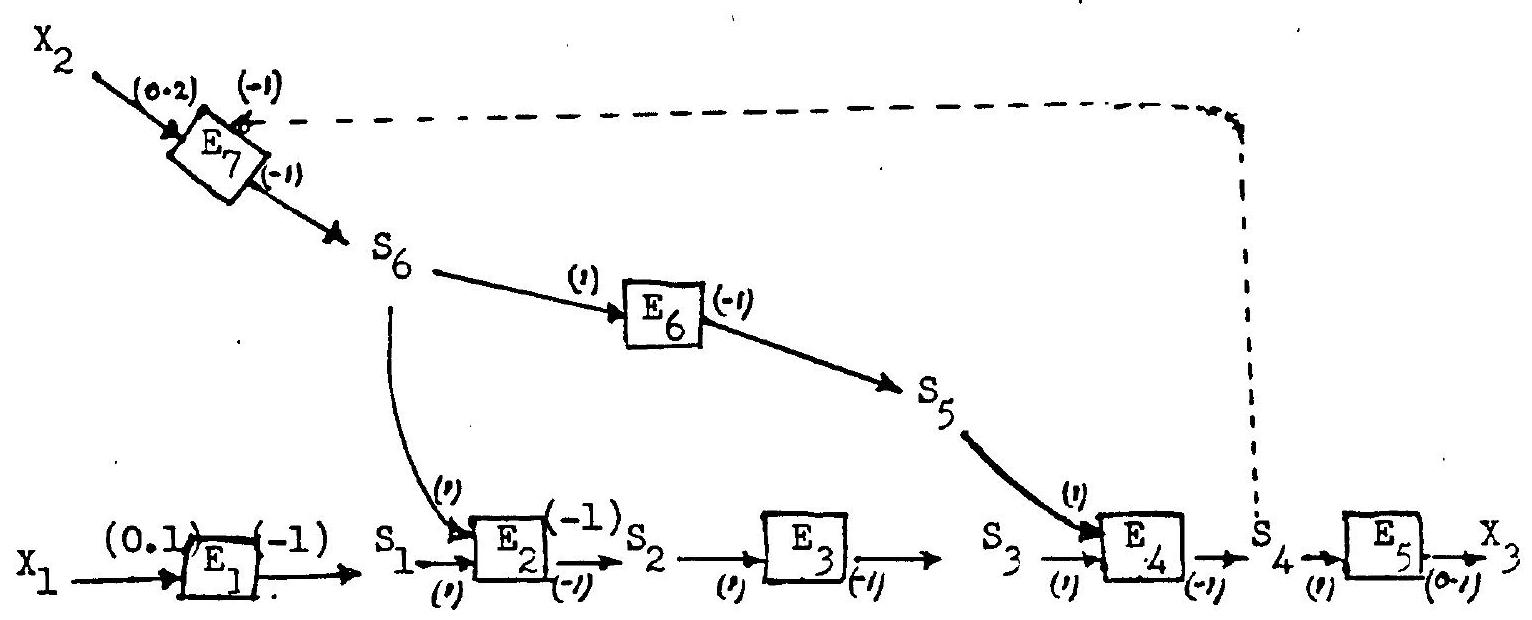
\includegraphics[max width=1\textwidth]{2023_01_30_a974a42f7b7381f3f940g-127(1)}
\end{center}

In this case the sequence of computation is:

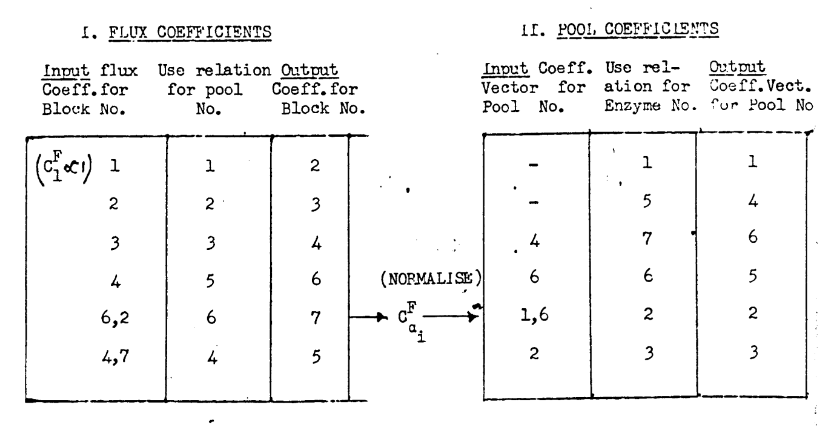
\includegraphics[max width=1.1\textwidth]{figure3_ExampII}

\begin{center}
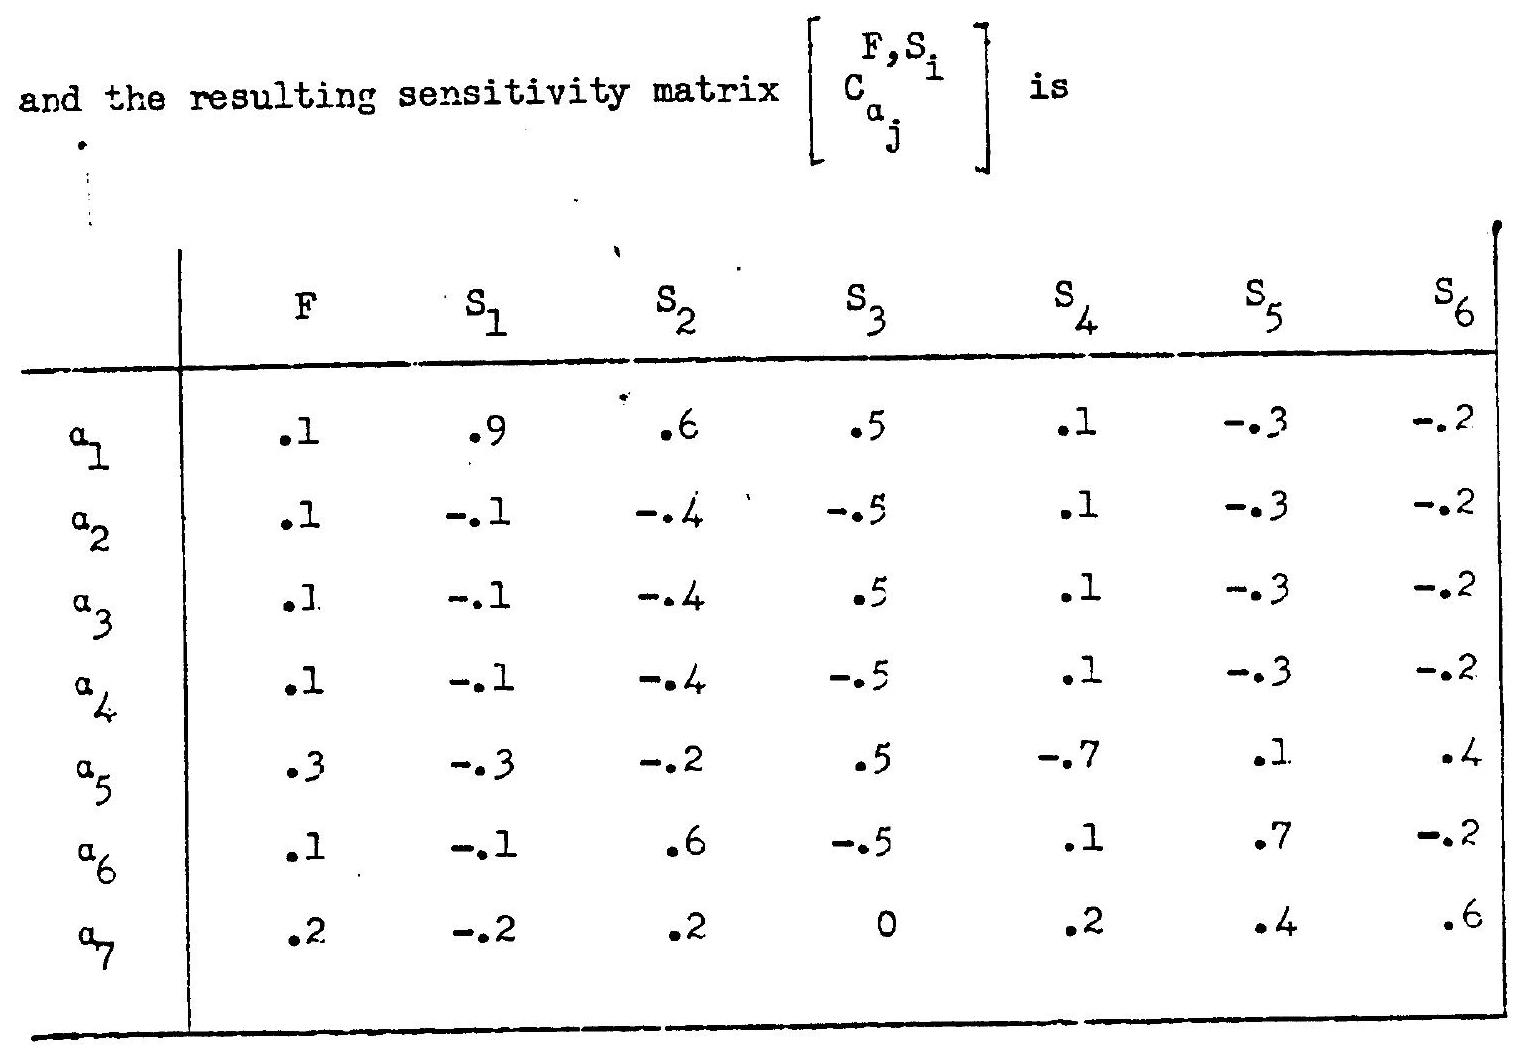
\includegraphics[max width=0.8\textwidth]{2023_01_30_a974a42f7b7381f3f940g-128}
\end{center}

{\bf\large EXAMPLE III: UREA TYPE CYCLE}

The two previous examples have considered 'uniflux' systems, that is systems characterised by $m-n=1$, and therefore possessing only one independent flux. For suck systems, once the $n$ relations of type (3.26) arising from pool modulations have been used, only one extra condition relating the coefficients was required and this condition was provided by the fact that $\sum C_{\alpha_{j}}^{F}=1$.

We now wish to consider systems with several independent fluxes where it will be necessary to use relations of type (3.33) which involve stoichiometric elasticities. As an example we will consider the system shown below which contains two independent fluxes $Y_{1}$ and $I_{2}$ and is similar to the urea cycle if $\mathrm{S}_{1}, \mathrm{S}_{2}, \mathrm{S}_{3}, \mathrm{S}_{4}$ stand respectively for ORN, CIT, ASA, ARG and $x_{2}$ is UREA. In order to define the stoichiometric elasticities it is necessary to know the ration $Y_{2} / Y_{1}$, i.e. the ratio of the flux round the cycle to the flux into protein and this is taken in this example to be $1 / 2$. As before all flux elasticities are taken to be $+1$ or $-1$ except for $\varepsilon_{1}^{6}$ which is taken as zero since this step is regarded as irreversible and $\varepsilon_{4}^{5}$ which is taken as $2 / 7$, again for arithmetic reasons.

\begin{center}
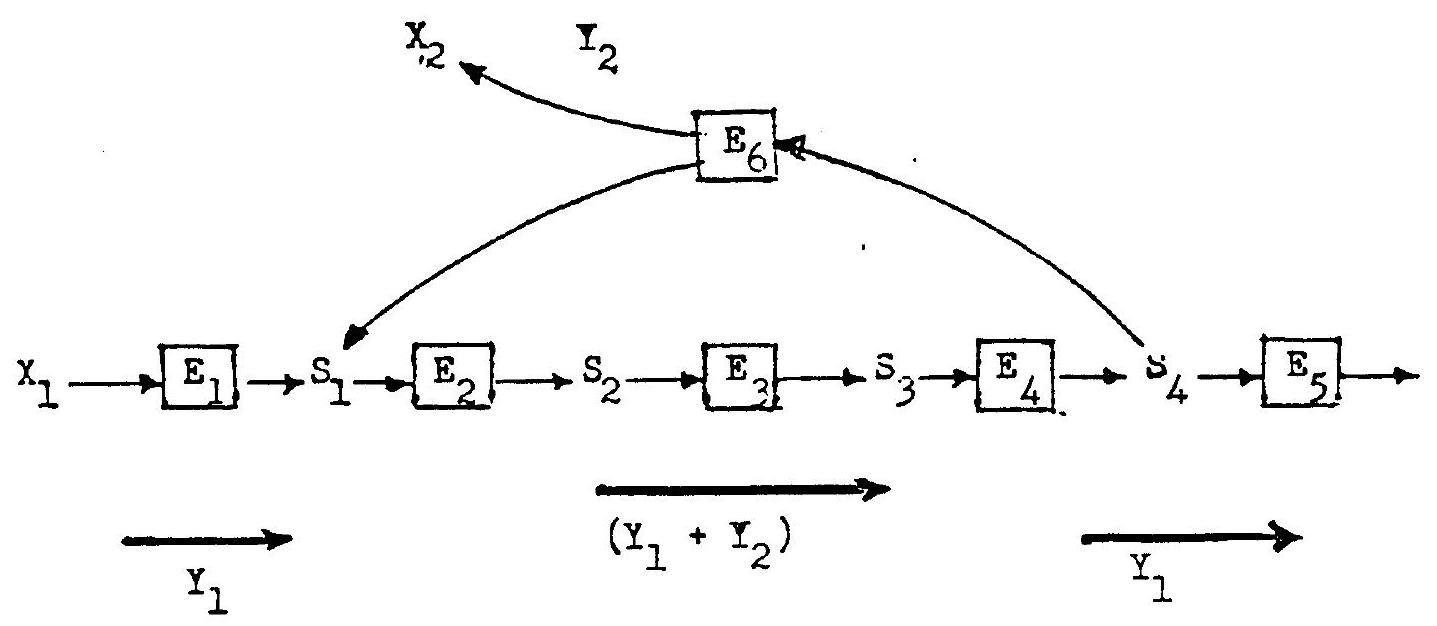
\includegraphics[max width=0.9\textwidth]{2023_01_30_a974a42f7b7381f3f940g-129}
\end{center}

Given then the ratio of the independent fluxes and the flux expression elasticities the computation of $\left[C^{Y_1,Y_2,S_i}_{\alpha_j}\right]$ proceeds as follows:

First of all we note that the stoichiometric elasticities of the local fluxes with respect to the independent fluxes can be written down by considering what fraction of a given flux is accounted for by a particular independent flux. This gives

$$ \varepsilon_{Y}^{F_j} \quad = [1, 2/3, 2/3, 2/3, 1, 0] $$

$$\mbox{ and } \varepsilon_{Y}^{F_2} \quad = [0, 1/3, 1/3, 1/3, 0, 1] $$

Considering first the sensitivity of the independent flux $Y_{1}$ to the separate blocks, let us suppose that $C^{Y_1}_1 = x$. Then the pool relationships for $S_{1} S_{2} S_{3}$ show that $C_{1}^{Y}=C_{2}^{Y_{1}}=C_{3}^{Y_{1}}=C_{4}^{Y_{1}}=x$ Suppose further that $C_{5}^{Y}=y$ and $C_{6}^{Y_{I}}
=2$

We can now use the relation for pool $\mathrm{S}_{4}$ to give
%
$$
(-1) \cdot x+(2 / 7) \cdot y+(1) \cdot z=0
$$
%
and the flux modulation relations of type (3.33), where modulation of $Y_{2}$ gives
%
$$
1 / 3 \cdot x+1 / 3 \cdot y+1 / 3 \cdot x+(1) \cdot z=0
$$
%
and modulation of $Y_{1}$ gives
%
$$
(1) \cdot x+2 / 3 \cdot x+2 / 3 \cdot x+2 / 3 \cdot x+(1) \cdot y=1
$$
%
These three equations are easily solved to yield
%
$$
x=0.1, y=0.7, z=-0.1
$$
%
or
%
$$
C_{\alpha j}^{Y_{1}}=[0.1, 0.1, 0.1, 0.1, 0.7, -0.1]
$$
%
A similar argument then yields $\mathrm{C}_{\alpha_j}^{\mathrm{Y_2}}=[0.35, 0.35, 0.35, 0.35, -1.05, 0.65]$ Before proceeding to discover the $C_{\alpha_j}^{S_{i}}$ using enzyme equations of type (3.35) it is necessary to know the sensitivity to each of the $\alpha_{j}$ of the flux carried by each enzyme. This has already been established for $E_{1}$, $E_{5}, E_{6}$, but we still require the sensitivities for $E_{2}, E_{3}, E_{4}$ which all carry the flux $\left(Y_{1}+Y_{2}\right)$.

This can be written down using the relation (3.10) proved earlier for a branched pathway.
%
$$C_{\alpha_{j}}^{\left(Y_{1}+Y_{2}\right)}=\frac{Y_{1}}{Y_{1}+Y_{2}} C_{\alpha_{j}}^{Y_{1}}+\frac{Y_{2}}{Y_{1}+Y_{2}} \cdot C_{\alpha_{j}}^{Y_{1}} = 2/3 C_{C_{\alpha_j}}^{Y_{1}}+1 / 3 C_{\alpha_{i}}^{Y_{2}}$$
%
or
%
$$\mathrm{C}_{\alpha_{j}}^{\left(Y_{1}+Y_{2}\right)} = [0.183, 0.183, 0.183, 0.183, 0.183, 0.116, 0.150]$$
%
From this point it is straightforward to obtain the $C_{\alpha_{j}}^{S_{1}}, C_{\alpha_{j}}^{S}, C_{\alpha_{j}}^{3} C_{\alpha_j}^{S}$ using successively the relation of type (3.35) for $\mathrm{E}_{1}, \mathrm{E}_{2}, \mathrm{E}_{3}, \mathrm{E}_{4} \cdot$ In this case it is important to remember that the term $C_{\alpha_{j}}^{F_{k}^{\prime}}$ in (3.35) refers in each case to tho flux carried by the particular enzyme which is involved.

\begin{center}
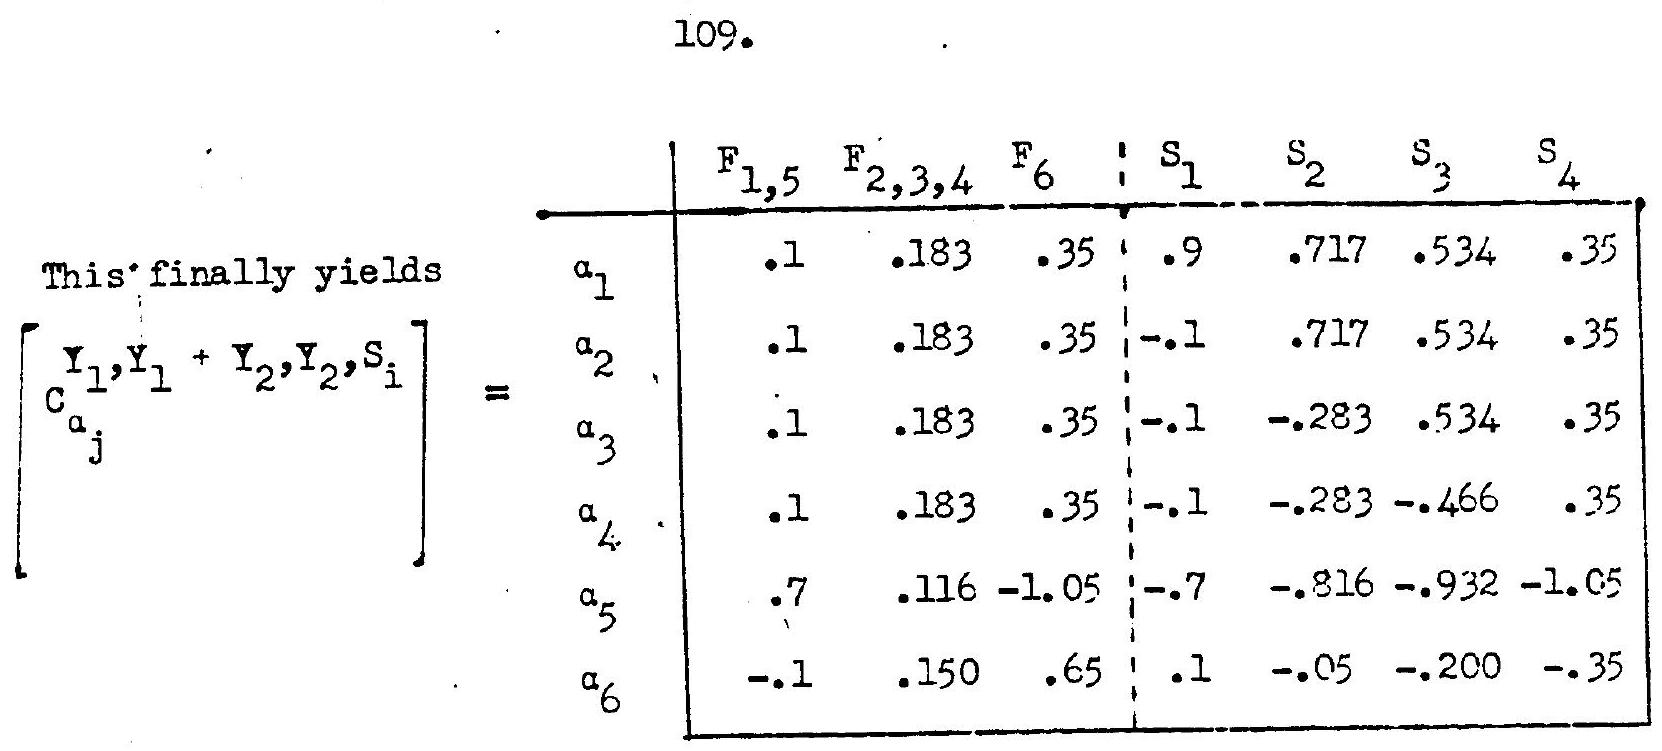
\includegraphics[max width=0.9\textwidth]{2023_01_30_a974a42f7b7381f3f940g-132}
\end{center}

Suppose now that it is required to know the sensitivity of the internal pools and fluxes to the level of $\mathrm{X}_{1}$. To obtain this we can use the relation (3.16) and, since the parameter $X_{1}$ only occurs in the block characterised by $\alpha_{1}$, we have
%
\begin{equation}
C_{X_{1}}^{M} = C_{\alpha_{1}}^{M_{1}} \cdot C_{X_{1}}^{F_{1}} = C_{\alpha_{1}}^{M} \cdot \varepsilon^{1}_{X_1}
\label{eqn:336}
\end{equation}
%
Noting from the diagram that the 1st block is rather saturated with respect to $X_{1}$, having an elasticity of only $0.1$, we can use the first row of the sensitivity matrix, together with $(3.36)$ to obtain
%
$$
\dot{C}_{X_{1}}^{F_{1,5}, F_{2, 3, 4}, F_{6}, S_{i}} = 0.01,\ 0.0183,\ 0.035,\ 0.09,\ 0.0717,\ 0.0534,\ 0.0351
$$
%
The above consideration shows that for a given S.S. system a knowledge of the relative values of the fluxes and of the elasticities of the separate flux expression at their working position is sufficient to determine the sensitivity matrix. In the examples given the task of calculating the sensitivity matrix from known. flux and stoichiometric elasticities was always straightforward. This was because the relatively simple `structure' of the systems under consideration gave rise in each case to a set of $m$ equations which could be solved by inspection.

\section{General limitations on coefficient values}

Previously we have seen that in certain uniflux systems we were able to state a general limit for the value of flux coefficients. These are systems in which all the $C_{\alpha_{j}}^{F}$ are necessarily + $v e$, when it follows that $0<C_{\alpha}^{F}<1$ for all j. No limitations were present for the pool coefficients. However, as soon as -ve coefficients become possible, either because of branching or perhaps, even in a uniflux system, when certain types of inhibition are operative, it is no longer clear that there are any such limits. Since it is not easy to consider this question in a general way we shall look instead at what limitation may exist in particular systems.

\section{Pool sensitivities in a chain of saturable enzymes}

Consider the simplest possible case; shown below, in which there is just one pool S. We wish to consider what limits are imposed on $C_{1}^{S}$.

\begin{center}
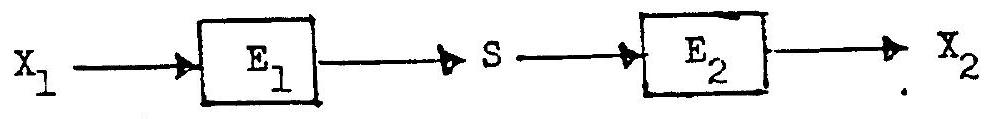
\includegraphics[max width=0.8\textwidth]{2023_01_30_a974a42f7b7381f3f940g-133(1)}
\end{center}

Clearly, by manipulating the relative quantity of $\mathrm{E}_{1}$ and $\mathrm{E}_{2}, \mathrm{S}$ car be anywhere within the range $X_{1} > S>  X_{2}$ (where the a are scaled concentrations taking account of the equilibrium constants). From the point of view of discussing the extreme, values of $C_{\alpha_{1}}^{S}$ and $C_{\alpha_{2}}^{S}$ we may take $S$ as being variable within this range.

Now using our previous theorem $(3.26)$ and denoting the elasticities by $\varepsilon_{S}^{1}$ and $\varepsilon_{S}^{2}$ we can write
%
$$
\mathrm{C}_{\alpha_{1}}^{F} \cdot \varepsilon_{S}^{1}+\mathrm{C}_{\alpha_{2}}^{F} \cdot \varepsilon_{S}^{2} = 0
$$
%
also $C_{\alpha_{1}}^{F} + C_{\alpha_{2}}^{F}=1$

so that $C_{\alpha_{1}}^{F}=\frac{\varepsilon_{S}^{2}}{\varepsilon_{S}^{2}-\varepsilon_{S}^{1}}$

and $\quad C_{\alpha_{1}}^{S} = C_{\alpha_{1}}^{F} / \varepsilon_{S}^{2}=\frac{1}{\varepsilon_{S}^{2}-\varepsilon_{S}^{1}}=-C_{\alpha_{2}}^{S}$

Clearly we car go no further without considering the form of the saturable rate expressions $f_{1}, f_{2}$ for the two enzymes. Let us assume that these are the simplest which will take saturation and reversibility fully into account, viz:
%
$$
\begin{aligned}
& f_{1}=\frac{X_{1}-S}{1+\frac{1}{M_{1}}+\frac{S}{M_{1}^{\prime}}} \\[6pt]
& f_{2}=\frac{S-X_{2}}{1+\frac{S}{M_{2}}+\frac{X_{2}}{M_{2}^{\prime}}}
\end{aligned}
$$
%
Where $M_{1}^{\prime}$ and $M_{2}^{\prime}$ are the `reverse' Michaelis constants. then using the formal relation, $C_{P}^{M_{1} / M_{2}}=C_{P}^{M_{1}}-C_{P}^{M_{2}}$, and finding the coefficients of the numerator and denominator by differentiation we have
%
\begin{align*}
\varepsilon_{S}^{1} &= C_{S}^{f_1} = -\left[\frac{S}{X_{1}-S}+\frac{S / M_{1}^{\prime}}{1 + X/M_{1} + S/M_{1}^{\prime}}\right] = -(a+b) \\
%
\mbox{ and } \varepsilon_{S}^{2} &= C_{S}^{f_{2}} = \left[\frac{S}{S - X_{2}}-\frac{S/M_{2}}{1+ S/M_{2} + X_{2}/X_{2}^{\prime}}\right] = (c-d)
\end{align*}

Where $a, b, c$, d represent the appropriate algebraic groupings. Clearly $a$ and $c$ represent components of the elasticity which depend mainly on `out of equilibriumness' of the reaction whereas $b$ and $d$ are concerned with the degree of saturation of the reaction. Inspection shows that
%
$$
0<a<\infty, \quad 1<c<\infty, \quad 0<b<1, \quad 0<d<1
$$
%
and that when the reaction steps are close to equilibrium the saturation term will be unimportant. Using this notation we have
%
$$
\begin{aligned}
C_{\alpha_{1}}^{S} &=\frac{1}{\varepsilon^{2}-\varepsilon^{1}} \\[4pt]
C_{\alpha_{1}}^{S} &=\frac{1}{a+b+c-d} \hspace{12PT}\mbox{and it is easy to establish} \\[4pt]
C_{\alpha_{1}}^{S} &>0
\end{aligned}
$$
%
Is there any upper bound for $\mathrm{C}_{\alpha_{1}}^{\mathrm{S}}$ ? The problem is to consider the maximum value of $C_{\alpha_{1}}^{S}$ for any values of $M_{1}, M_{1}^{\prime}, M_{2}, M_{2}^{\prime}$ and any value of $S$ in the range $X_{1}> S > X_{2}$

We require a `minimum' of $(a+b+c-d)$ and this will be so when

\begin{enumerate}[label=(\roman*),parsep=-3pt]
\item d is maximal, $=1$, i.e. $E_{2}$ fully saturated

\item b is minimal, $=0$, i.e. $E_{1}$ fully unsaturated
\end{enumerate}

This merely requires sufficiently extreme values of $M_{1}^{\prime}$ and $M_{2}$ and can be satisfied regardless of the value of S.

(iii) S lies at a value which will minimise $(a+c)$

$\displaystyle \mbox{Now} \quad a+c=\frac{S}{X_{1}-S}+\frac{S}{S-X_{2}} $

and it can be shown that the minimum occurs at $S = \sqrt{X_{1} \cdot X_{2}}$ So that
%
$$
\begin{aligned}
\left(C_{\alpha_{1}}^{\mathrm{S}}\right)_{\max } & =\frac{1}{(a+c)_{\min}+0-1} \\[6pt]
& =1 / 2\left(\sqrt{\frac{\mathrm{X}_{1}}{\mathrm{X}_{2}}}-1\right)
\end{aligned}
$$
%
At this maximum position the value of the flux coefficient is
%
$$
\mathrm{C}_{\alpha_{1}}^{\mathrm{F}} = 0.5
$$
%
Thus we have established that in the absence of any knowledge other the than a general form for the saturable expression and the values of $X_{1}, X_{2}$
%
$$
0 < C_{\alpha_{1}}^{S} < 1/2\left(\sqrt{\frac{X_{1}}{X_{2}}}-1\right)
$$
%
Clearly then if $X_{1} \gg X_{2}$ there is no effective limit to the value of $C_{\alpha_{1}}^{S}$ and we may expect that under certain circumstances very large values of pool coefficients could occur.

In particular a large pool coefficient appears likely whenever a saturated and almost irreversible enzyme appears at the end of a chain and when the flux control is shared equally between it and the rest of the chain.

\section{Pool sensitivities in a chain of linear enzymes}

In the case of two linear enzymes an almost identical argument applies, except that the saturation components of the elasticities are absent so that
%
$$
C_{\alpha}^{S}=\frac{1}{a+c}
$$
%
Once again the minimum occurs when $S=\sqrt{X_{1} X_{2}}$

\medskip
and gives the result $0 < C_{\alpha}^{S}<\frac{\sqrt{X_{1}}-\sqrt{X_{2}}}{\sqrt{X_{1}}+\sqrt{X_{2}}}$, so that $C_{\alpha}^{S} < 1$

\medskip
the value of $C_{\alpha_{1}}^{F}$ at this maximum is $C_{\alpha_{1}}^{F} \bumpeq \frac{\sqrt{X_{1}}}{\sqrt{X_{1}}+\sqrt{X_{2}}}$

\medskip
$ \displaystyle \text { For example if } \mathrm{X}_{1}=100, \mathrm{X}_{2}=1,\left(C_{\alpha}^{S}\right)_{\max }=\frac{10 -1}{10+1}=82 \% $

\medskip
$ \displaystyle \text { at which position } C_{\alpha_{1}}^{F} \bumpeq \frac{10}{10+1}=90 \% \text { This indicates that the } $

\medskip
$ \displaystyle \text { result } C_{\alpha_{1}}^{F}=0.5 $  for the saturable case is not general and, more importantly, we have demonstrated that in a chain of linear enzymes the  pool coefficients are strictly bounded.


\section{Flux coefficients}

The results just proved for pool coefficients can be used to show that in systems with branching, that is with more than one independent flux, there is no a priori limit on the values of flux coefficients as there is for a straight chain of enzymes.

Consider the branching system shown below, where $E_{1}$ and $E_{2}$ may be saturable enzymes.

\begin{center}
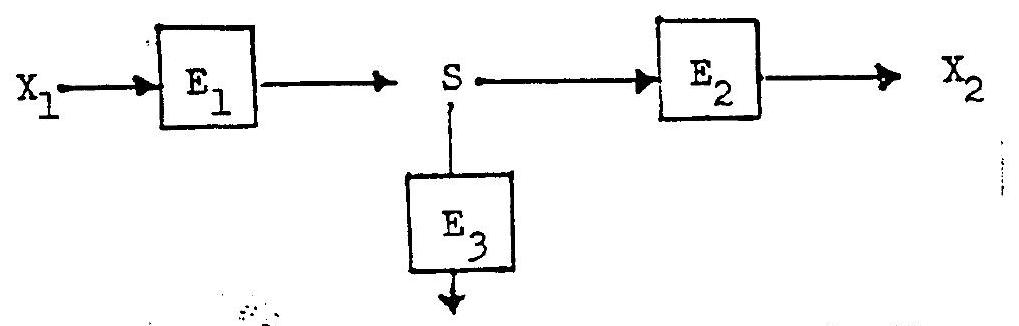
\includegraphics[max width=0.7\textwidth]{2023_01_30_a974a42f7b7381f3f940g-138}
\end{center}

Let us suppose that the enzyme $E_{3}$ is effectively linear and irreversible and that the flux through it, $F_{3}$, is small compared with the fluxes $F_{1}$ and $F_{2}$ in the main pathway.

Under these circumstances it follows that $\mathrm{C}_{\alpha_{1}}^{\mathrm{F}_{3}} \bumpeq \mathrm{C}_{\alpha_{1}}^{\mathrm{S}}$ and, from the result just proved for a chain of two saturable enzymes, also
%
$$
\left(C_{\alpha_{1}}^{S}\right)_{\max } \bumpeq 1/2\left(\sqrt{\frac{X_{1}}{X_{2}}}-1\right)
$$
%
Thus
%
$$
\left(C_{\alpha_{1}}^{F_3}\right)_{\max} \bumpeq 1/2\left(\sqrt{\frac{X_{1}}{X_{2}}}-1\right)
$$
%
This demonstrates that very large + or -ve values of flux coefficients are possible in a branching system which contains saturable enzymes.

It will be noticed, however, that this result is for the coefficient of a flux with respect to an enzyme not directly in the pathway carrying the flux. In fact it is often possible to identify, within a larger system, major pathways which carry a flux large by comparison with any branches from them. The coefficients of the flux ir: such major pathways with respect to the enzymes actually in them will under normal circumstances still satisfy the limitation $0 < C_{\alpha}^{F} < 1$

\section{`Diagnostics' for rate control in non-linear systems}

In $\mathrm{Ch}$ I it was shown, for a sequence of linear enzymes, that the difference in pool levels across enzymes in a chain was Iror.rrtional to their respective flux coefficients, $C_{\alpha_{i}}^{F}$, provided the pool concentrations were scaled to take account of the product of equilibrium constants along the chain. Thus the pattern of scaled pool levels at the S.S. could be used as a simple diagnostic for rate control. We now wish to consider how this simple diagnostic for rate control in a chain of enzymes will be altered when allowance is made for enzymes having saturable rate expressions.

\begin{center}
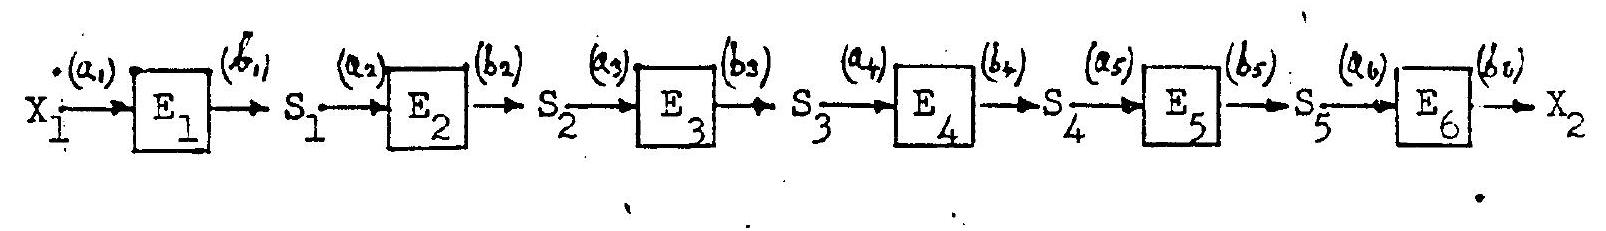
\includegraphics[max width=\textwidth]{2023_01_30_a974a42f7b7381f3f940g-140}
\end{center}

Such a system is shown above and the substrate and product elasticities `a' and `b' respectively, are written next to each enzyme using the appropriate suffixes. By using the pool modulation relations (3.26) and arbitrarily taking the unnormalised value of the 1st flux coefficient, $C_{1}$, as $1/a_{1}$ we can show that:
%
\begin{equation}
\left[C_{1}, C_{2}, C_{3}, \ldots\right] \propto\left[\frac{1}{a_{1}}, \quad \frac{1}{a_{2}}\left(-\frac{b_{1}}{a_{1}}\right), \quad \frac{1}{a_{3}}\left(-\frac{b_{1}}{a_{1}}\right)\left(-\frac{b_{2}}{a_{2}}\right), \ldots \ldots \ldots\right]
\label{eqn:339}
\end{equation}
%
This shows that the elasticities of a given enzyme, say $E_{3}$, affect its own coefficient directly through the factor $\frac{1}{a_{3}}$ and indirectly by multiplying all terms 'downstream' from it by the factor $\left(-\frac{b_{3}}{a_{3}}\right)$. In order to proceed further we must now assume the simplest rate expression which will adequately represent the saturability and reversibility of the typical step shown below.

\begin{center}
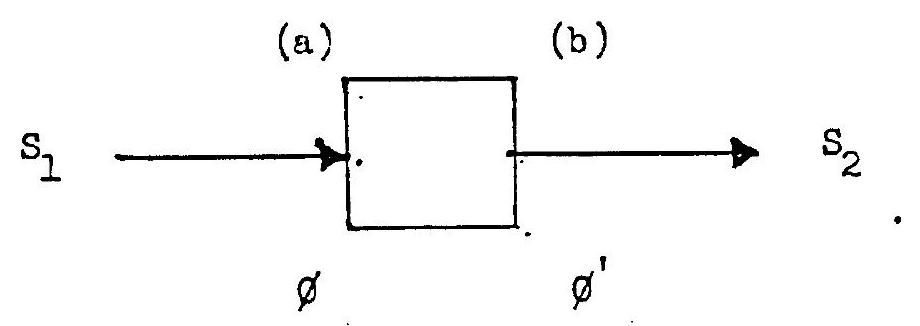
\includegraphics[max width=0.9\textwidth]{2023_01_30_a974a42f7b7381f3f940g-140(1)}
\end{center}

If $S_{1}$ and $S_{2}$ are suitably scaled so that the equilibrium constant is eliminated such an expression will be
%
\begin{equation}
F=\frac{\frac{\mathrm{V}}{\mathrm{M}}\left(\mathrm{S}_{1}-S_{2}\right)}{I+\frac{S_{1}}{M}+\frac{S_{2}}{M^{\prime}}}=\frac{\frac{\mathrm{V}^{\prime}}{M^{\prime}}\left(S_{1}-
S_{2}\right)}{1+\frac{S_{1}}{M}+\frac{S_2}{M^{\prime}}}
\label{eqn:339}
\end{equation}
%
In this expression $V$ and $V^{\prime}$ represent the forward and reverse maximum velocities of the enzyme while $M$ and $M^{\prime}$ represent Michaelis constants for the substrate $S_{1}$ and the product $S_{2}$ respectively.

Using this rate equation it is now possible to write down the elasticities `a' and `b' with respect to $S_{1}$ and $S_{2}$ as
%
\begin{equation}
\begin{aligned}
& a =\frac{S_{1}}{S_{1}-S_{2}}-\frac{\frac{S_{1}}{M}}{1+\frac{S_{1}}{M}+\frac{S_{2}}{M^{\prime}}}=\frac{S_{1}}{S_{1}-S_{2}}- \phi \\
& b =-\frac{S_{2}}{S_{1}-S_{2}}-\frac{\frac{S_{2}}{M^{\prime}}}{1+\frac{S_{1}}{M}+\frac{S_{2}}{M^{\prime}}}=-\frac{S_{2}}{S_{1}-S_{2}}-\phi^{\prime}
\end{aligned}
\label{eqn:339}
\end{equation}
%
Where the terms $\phi$ and $\phi^{\prime}$, arising from the saturation property of the rate expression with regard to $S_{1}$ and $S_{2}$ respectively, are both positive and can be seen to satisfy the inequality $\left(\phi+\phi^{\prime}\right) < 1$. The latter condition means that it is impossible for  $\phi$ and $\phi^{\prime}$  to approach
their maximum values of unity simultaneously. The elasticities of (3.39) can be written as their 'linear' parts multiplied by correction
factors which differ from unity when saturation effects are important, thus
%
\begin{equation}
\begin{aligned}
& a = \frac{S_{1}}{S_{1}-S_{2}}\left(1-\phi \frac{S_1-S_2}{S_1}\right) \\
& b = -\frac{S_{2}}{S_{1}-S_{2}}\left(1+\phi^{\prime} \frac{S_{1}-S_{2}}{S_{2}}\right)
\end{aligned}
\label{eqn:340}
\end{equation}
%
Inspection of these correction factors indicates that the effect of saturation depends not only on the terms $\phi$ and $\phi^{\prime}$ but also on the equilibrium situation around the enzyme. For example if the `out of equilibrium ration, $\frac{S_{2}}{S_{1}}$, is close to unity the correction will be negligible even though one or other of the saturation terms may be at its maximal value.

The factors $\left(\frac{1}{a}\right)$ and $\left(-\frac{b}{a}\right)$ which occur for each enzyme in (3.37) can also be written as a `linear' part multiplied by correction factors $\beta$ and $\gamma$ respectively. Thus,
%
\begin{equation}
\frac{1}{a}=\frac{S_{1}-S_{2}}{S_{1}} \cdot \frac{1}{\left(1-\phi \frac{S_{1}-S_{2}}{S_{1}}\right)}=\frac{S_{1}-S_{2}}{S_{1}} \cdot \beta
\label{eqn:341}
\end{equation}
%
$$\left(-\frac{b}{a}\right)=\frac{S_{2}}{S_{1}} \cdot \frac{\left(1+\phi^{\prime} \frac{S_{1}-S_{2}}{S_{2}}\right)}{\left(1-\phi \frac{S_{1}-S_{2}}{S_{1}}\right)}=\frac{S_{2}}{S_{1}} \cdot \gamma
$$
%
Using the relation (3.41) with appropriate suffixes we can write (3.37) as
%
\begin{equation}
\left[C_{1}, C_{2}, C_{3}, \cdots\right] \cdot \left[\frac{X_1-S_1}{X_1} \cdot \beta_1, \frac{S_1-S_2}{X_1} \cdot \beta_2 \cdot \gamma_1, \frac{S_2-S_3}{X_1} \cdot \beta_3 \cdot \gamma_1 \cdot \gamma_2, \cdots \cdot\right]
\label{eqn:342}
\end{equation}
%
In the linear case, when $\phi=\phi^{\prime}=0$ for all enzymes, all $\beta$ and $\gamma$ terms in (3.42) are unity and the successive flux coefficients are just proportional to the scaled pool differences, confirming the result of CH.I. When however saturation effects are important it will be necessary to have some estimate of the factors $\beta$ and $\gamma$ in addition to the ratios of scaled pool levels which were a sufficient diagnostic in the linear case.

One possible way of estimating. the correction factor $\beta$ for an enzyme would be to use the definition, from (3.41), of
%
\begin{equation}
\beta=\frac{1}{1-\phi \frac{S_{1}-S_2}{S_1}}=\frac{1}{1-\frac{\frac{S_1}{M}}{1+\frac{S_1}{M}+\frac{S_2}{M^{\prime}}} \times\left(\frac{S_1-S_2}{S_1}\right)}
\label{eqn:341}
\end{equation}
%
However this would involve making a close study of each enzyme, to determine the Michaelis constants $M$ and $M^{\prime}$, and also a knowledge of \underline{absolute} pool levels rather than ratios.

Alternatively we may note from (3.38) that
%
$$\frac{F}{V}=\left(\frac{S_1}{M} \big/\left(1+\frac{S_1}{M}+\frac{S_2}{M^{\prime}}\right)\right) \quad \times \quad \frac{S_1-S_2}{S_1} = \phi \cdot \frac{S_1-S_2}{S_1}$$
%
so that
%
\begin{equation}
\beta=\frac{1}{1-\phi \frac{S_{1}-S_{2}}{S_{1}}}=\frac{1}{1-\frac{F}{V}}
\label{eqn:344}
\end{equation}
%
and similarly we can show that
%
\begin{equation}
 \gamma = \frac{1 + \frac{F}{V^\prime}}{1-\frac{F}{V}}
\label{eqn:345}
\end{equation}
%
Thus estimates for $\beta$ and $\gamma$ can be made by measuring the flux $F$ for unit weight of the organism and dividing it by the maximum activity in the forward and reverse directions of the enzyme extracted from unit weight, forming the required factors $\frac{F}{V}$ and $\frac{F}{V^\prime}$.

In principle, then, $\dot{a}$ knowledge for each enzyme of pool ratios and of in vivo flux against maximum flux can be used to diagnose relative flux control using the following relation, obtained by substituting the expressions (3.44) and (3.45) for $\beta$ and $\gamma$ into (3.42). Thus we have
%
\begin{equation}
\begin{split}
  \left[C_{1}, C_{2}, C_{3}, \cdots\right] &\propto  \left[ \frac{X_{1}-S_{1}}{X_{1}} \frac{1}{\left(1-\frac{F}{V_{1}}\right)},
%
\frac{S_1-S_2}{X_1}  \frac{1}{\left(1-\frac{F}{V_2}\right)}  \frac{\left(1+\frac{F}{V_1}\right)}{\left(1-\frac{F}{V_1}\right)}, \right. \\[7pt]
%
&\left. \frac{S_2-S_3}{X_0} \frac{1}{\left(1-\frac{F}{V_3}\right)}\left(\frac{1+\frac{F}{V_{1}^{\prime}}}{1-\frac{F}{V_1}}\right), \ldots \hspace{14pt}  \right]
\end{split}
\label{eqn:346}
\end{equation}
%
The pattern of pools around an enzyme in fact imposes limits on the values which $\beta$ and $\gamma$ can assume. Thus inspection of the expression (3.44) reveals that, for a given value of $S_{1}$ and $S_{2}, \beta$ will be a maximum when the forward saturation, $\phi$, approaches unity and a minimum when $\phi$ approaches zero. So that
%
\begin{equation}
1 < \beta < \frac{S_{1}}{S_{2}}
\label{eqn:347}
\end{equation}
%
A similar but rather more complex argument for (3.45) shows that $\gamma$ approaches a maximum when $\left(\phi+\phi^{\prime}\right)$ approaches unity, irrespective of the separate values of $\phi$ and $\phi^{\prime}$. So that we also have
%
\begin{equation}
1 < \gamma < \frac{S_{1}}{S_{2}}
\label{eqn:348}
\end{equation}
%
When attempting to estimate flux coefficients from a given set of pool data a useful first step is to take them as proportional to scaled pool differences, using the linear enzyme assumption. If additional evidence indicates that an enzyme may be saturated the effect of allowing for this will be to increase the value of the coefficient of all enzymes downstream from it by the common factor, $\gamma$, and also to increase its own coefficient by the factor $p$, which will be greater than unity and may approach $\frac{S_1}{S_2}$ if the saturation is predominantly forward. The inequalities established for $\beta$ and $\gamma$ indicate that it will only be important to allow for saturation effects at steps having a large 'out of equilibrium' ratio, $\frac{S_1}{S_2}$.

For example if all enzymes were known to be saturated from in front, in the sense that they had $\phi=1$, the application of (3.42) would give
%
$$
\left[C_1, C_2, C_3, C_4, C_5, C_6\right] \propto\left[\frac{X_1-S_1}{S_1}, \frac{S_1-S_2}{S_2}, \frac{S_2-S_3}{S_3}, \frac{S_3-S_4}{S_4}, \frac{S_4-S_5}{S_5}, \frac{S_5-X_2}{X_2}\right]
$$
%
Clearly if $\frac{X_1}{X_2}$ is close to unity, that is the whole chain is close to equilibrium, then a prediction based on the linear assumption will be good. If, however, $\frac{X_1}{X_2}$, is large then enzymes further down the chain may have much greater coefficients than would be expected on a linear hypothesis.

In particular whenever $X_1$ is close to zero, rendering the last step irreversible, the degree of saturation of the last step becomes of critical importance.

\section{Pools attenuate with metabolic distance}

{\bf Does the effect on pools attenuate with metabolic distance from the site of a modulation?}

We are now in a position to consider this question, for our straight chain of non-linear enzymes, taking the modulation to act on the quantity of some enzyme within the chain and 'metabolic distance' to be the number of enzymes between the modulation and the pool in question. Show below is a typical enzyme in the chain, not subject to modulation, and across which such 'attenuation' might occur once again, `a' and `b' indicate the appropriate elasticities.

\begin{center}
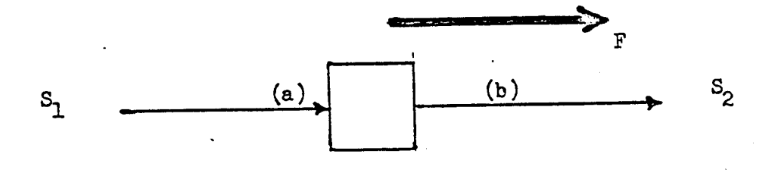
\includegraphics[scale=0.8]{figure3_Chain1.png}
\end{center}

Denoting the coefficients of the pools and of the flux, F, with respect to the remote modulated enzyme as $C_{1}, C_{2}$ and $C_{F}$ respectively it is convenient to consider $C_{1}$ and $C_{2}$ in terms of their deviations $\Delta_{1}$ and $\Delta_{2}$ from $C_{F}$, the flux coefficient $C_{F}$ being, of course, the same no matter which enzyme in the chain is considered. Thus
%
$$
C_{1} = C_{F}+\Delta_{1} \quad \text { and } \quad C_{2}=C_{F} + \Delta_{2}
$$
%
We can then discover whether $\Delta$ increases or decreases on passing through a particular enzyme by applying an enzyme relationship of type (3.35), which gives
%
$$
C_1 = \left(C_F - b \cdot C_2\right) / a
$$
or
%
$$ C_F+\Delta_1 = \left(C_F-b\left(C_F+\Delta_2\right)\right) / a $$
%
so that
%
\begin{equation}
\Delta_1 = A \Delta_2 + B C_F
\label{eqn:349}
\end{equation}
%
where
%
$$
A = \left(-\frac{b}{a}\right) \text { and } B=\frac{(1-b-a)}{a}
$$
%
Clearly the increase or decrease of $\Delta$ on passing through an enzyme will depend on the values assumed by the factors $A$ and $B$. Assuming the non linear enzyme to be of the same form as in the last section we can use the results obtained there to discover the limits on the numbers $A$ and $B$ in terms of the pools $S_{1}$ and $S_{2}$ surrounding the given enzyme.
%
$$
\text { Thus we had, from }(3.41) \text {, that } A=\left(-\frac{\mathrm{b}}{\mathrm{a}}\right)=\frac{\mathrm{S}_{2}}{\mathrm{S}_{1}} \cdot \gamma
$$
%
and using the inequality (3.48), for $\gamma$, this yields
%
\begin{equation}
\frac{S_{2}}{S_{1}} < A < 1
\label{eqn:350}
\end{equation}
%
Also we have from (3.39) that
%
$$
(1-a-b)=1-\frac{S_{1}}{S_{1}-S_{2}}+\frac{S_{2}}{S_{1}-S_{2}}+\left(\phi+\phi^{\prime}\right) $$
%
which simplifies to
%
$$
(1-a-b) = \phi + \phi^{\prime}
$$
%
$ \displaystyle \text { using }(3.41) \text { to provide the factor }\left(\frac{1}{a}\right) \text { this gives } $
%
$$
B = \frac{1-a-b}{a}=\left(\phi+\phi^{\prime}\right) \cdot \frac{\left(S_{1}-S_{2}\right)}{S_{1}} \cdot \beta
$$
%
and finally using the inequality (3.47) for $\beta$ together with the fact that maximum $\beta$ coincides with maximum $\phi$ we have
%
\begin{equation}
0 < B < \frac{S_{1}-S_{2}}{S_{2}}
\label{eqn:351}
\end{equation}

In both of these inequalities the minimum value occurs when the enzyme is `linear', the maximum when it is fully saturated.

Referring to the chain of enzymes indicated in the diagram below, where the disturbance acts at $E_{4}$, it is now possible to see under what circumstances attenuation of the disturbance might be expected, by using the relation (3.49) together with the inequalities just established for $A$ and $B$.

\begin{center}
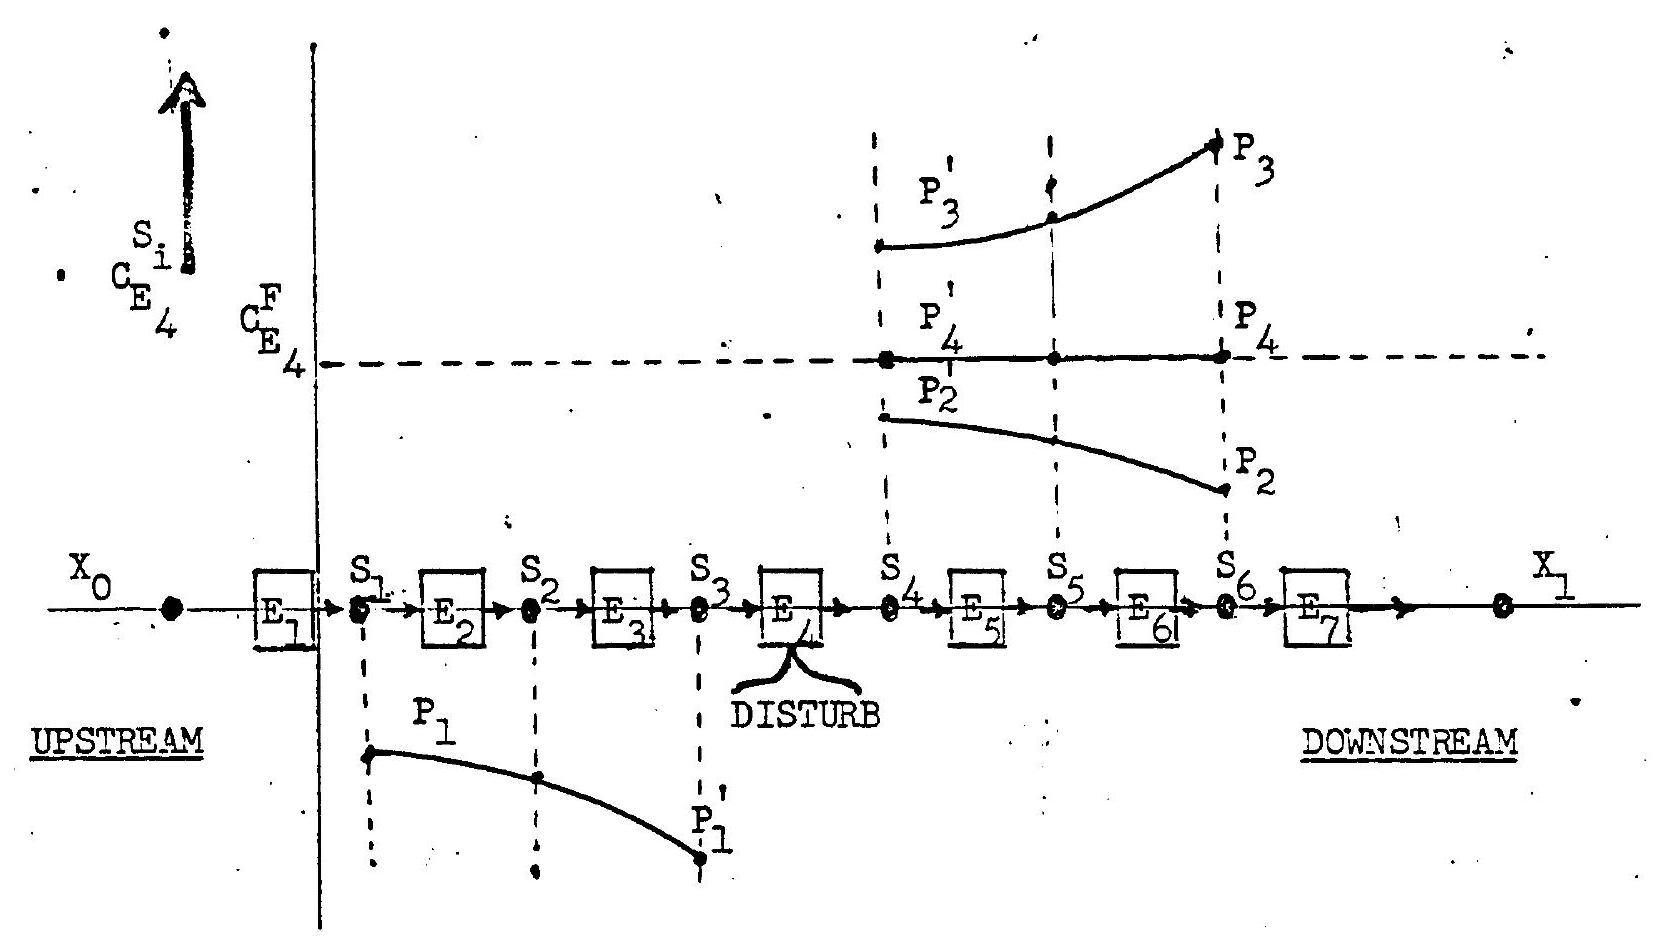
\includegraphics[max width=\textwidth]{2023_01_30_a974a42f7b7381f3f940g-150}
\end{center}

Thus, on the upstream side of the disturbance it is clear that all the $\Delta S$ must be -ve and that the effect of moving through any of the enzymes $E_{3}, E_{2}, E_{1}$ must be to `shrink' this difference from the dotted line, $C_{F}$, by the factor $A$ and then to further add the positive quantity B. $C_{F}$. Thus whatever the condition of the enzymes upstream from $E_{4}$ they will always attenuate the fractional disturbance in the pools according to a curve such as $P_{1} P_{1}^{\prime}$ on the diagram.

Downstream such a result does not necessarily apply. What actually happens will depend on the saturation and `out of equilibriumness' of the separate enzymes.

Let us suppose, for example, that enzymes $\mathrm{E}_{5}, \mathrm{E}_{6}$ are linear. In this case the factor A, for each enzyme, is of the form $\frac{S_{2}}{S_{1}}$ and the factor $B$ will be zero. Applying the relation $(3.49)$ to enzymes 6 and 5 therefore gives
%
$$
\Delta_{5}=\left(\frac{S_{6}}{S_{5}}\right) \cdot \Delta_{6}\hspace{6pt} \text { and } \hspace{6pt} \Delta_{4}=\left(\frac{S_{5}}{S_{4}}\right) \cdot \Delta_{5} \text { This shows that }
$$
%
if $C_6^{\mathrm{E_4}} < C^F_{E_4}$, that is $\Delta_{6}$ is -ve, then a curve $P_{2} P_{2}^{\prime}$ representing attenuation will be the result. If, however $C_{E_4}^{S_6} > C_{E_4}^{F}$ a curve $\mathrm{P}_{3} \mathrm{P}_{3}^{\prime}$, representing amplification of the disturbance will result, A third possibility is that $\mathrm{C}_{\mathrm{E_4}}^{\mathrm{S}_{6}} = \mathrm{C}_{E_4}^{\mathrm{F}}$ in which case the effect is to give a neutral curve $P_{4} P_4^{\prime}$ The sign of $\left(C_{E_4}^{S_6} - C_{E_4}^{F}\right)$, which determines these possibilities, depends on the condition of the last enzyme and can be considered by applying a relationship of type (3.35) to enzyme $\mathrm{E}_{7}$. This gives
%
$$
a_{7} \cdot C_{E_4}^{S_{6}} = C_{E_4}^{F}
$$
%
and hence
%
$$
C_{E_4}^{S_{6}}-C_{E_4}^{F} = C_{F}\left(\frac{1}{a}-1\right)=C_{F} \cdot Y
$$
%
where $Y$ stands for the factor $\left(\frac{1}{a}-1\right)$.

Using relationship $(3.41)$ to replace $\frac{1}{a}$ along with the inequality $1 < \beta < \frac{S_{1}}{S_{2}}$ and noting that $Y$ is a maximum when $\beta$ is a maximum we can show that
%
$$
-\frac{\mathrm{X}_{1}}{\mathrm{S}_{1}} < \mathrm{Y} < \frac{\left(\mathrm{S}_{1}-2 \mathrm{X}_{2}\right)}{\mathrm{X}_{2}}
$$
%
This result shows that whenever $S_{1}>2 X_{1}$ it is possible for $Y$ to be either negative or positive so that either an amplifying or an attenuating curve can result. The existence of the attenuating type curve, $P_{2} P_{2}^{\prime}$, or of the amplifying type, $P_{3} P_{3}^{\prime}$, depending on the degree of saturation of the last enzyme.

A further point is that if the enzymes $E_{5}$ and $E_{6}$ are not linear then there need be no steady gradient at all. However, it is never possible for $C_{E_4}^{S_i}$ to descend below $C_{E_4}^{F}$ if we start with $\mathrm{C}_{\mathrm{E_4}}^{\mathrm{S}_{6}} > \mathrm{C}_{\mathrm{E}_{4}}^{\mathrm{F}}$ and proceed in the direction $\mathrm{S}_{6}, \mathrm{S}_{5}, \mathrm{S}_{4}$.


\section{In vivo destination of elasticities}

{\bf In vivo destination of elasticities as a means of discovering the sensitivity matrix}

We return now to the idea, proposed earlier in this chapter, that it may be possible to estimable the elasticities of system components around their working position on the basis of only. a limited number of in vivo parameter modulation S.S. experiments. Having obtained estimates of these elasticities it will then be straightforward to compute the sensitivity matrix $\left[C_{\alpha_{j}}^{F, S_{i}}\right]$ using the methods already outlined.

Basically the idea is that by using our information about the `structure: of the system, that is its' metabolic diagram together with all control information, and measuring only the ratios of observed small fractional responses of type $\frac{\Delta S}{S}$ and $\frac{\Delta F}{F}$ consequent on the in modulation of only a few environmental parameters it will be possible to arrive at a complete sensitivity matrix.

Such an approach to discovering the sensitivity matrix involves no absolute measurements whatsoever, assumes nothing about the form of the rate-expression except what is implied in the structure diagram, and involves only a small number of parameter modulations which can . often be external and therefore easily manipulable. Furthermore, since the required \underline{ratios} of small fractional responses do not depend on the details of a parametric modulation but only on its location it becomes relatively straightforward to use revertants, with small but measurable effects, as a source of modulation when the structure of the system necessitates manipulation of genetic parameters.

The direct experimental methods for estimating coefficients outlined earlier, although sharing the above advantage of being in vivo and measuring only fractional responses, contrast unfavourably because they involve complicated experiments to produce exactly known modulations of genetic parameters and because it would be necessary to repeat this laborious procedure for each block in the system if we are to produce a sensitivity matrix.

Similarly the `diagnostic' approach, although perhaps useful for a quick appraisal from pool levels of possible rate controlling steps, appears even more unfavourable. Thus it involves assumptions about the form of rate-expression which are based on in vitro studies and may be of dubious relevance to the actual in vivo working of the enzyme. In addition it is difficult to determine the necessary factors to produce `scaled' pool values and the method itself is not easy to extend beyond the straight chain case just presented.

Assume then that the structure of a problem is tentatively known, that the system under study has three external pools and that a particular enzyme in it, $\mathrm{E}_{10}$, has non zero elasticity for the three pools, $S_{1}, S_{2}, S_{3}$ as shown below.

\centerline{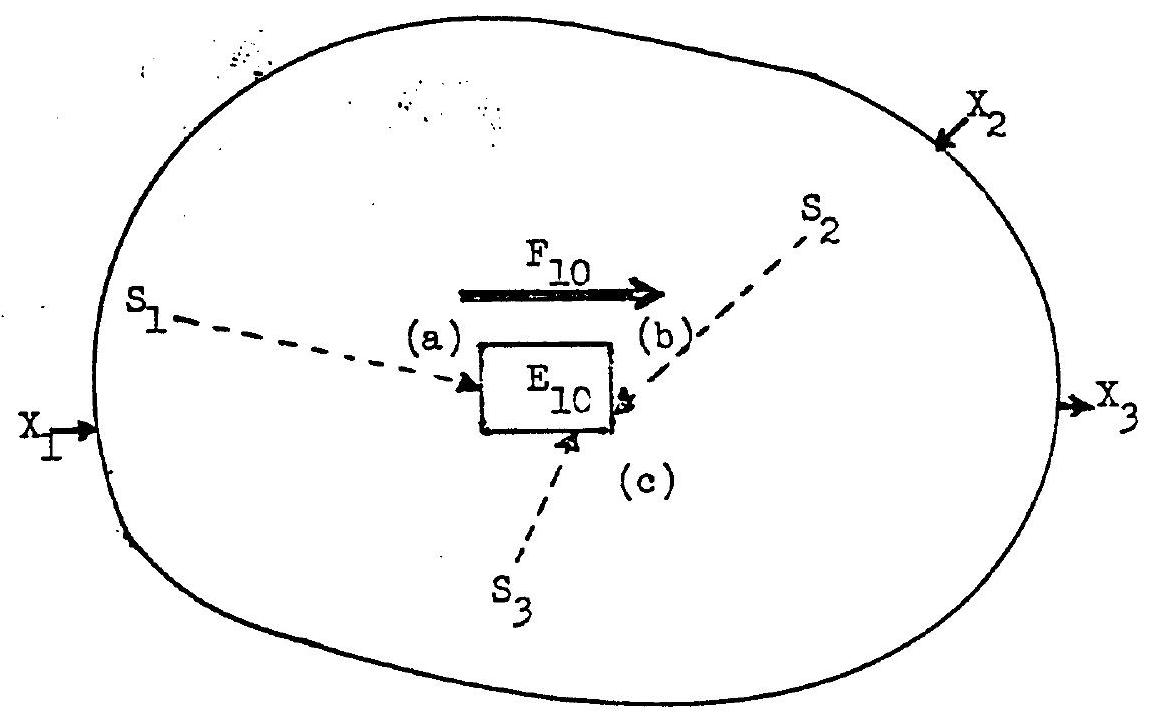
\includegraphics[max width=0.56\textwidth]{2023_01_30_a974a42f7b7381f3f940g-154}}


Denoting the elasticities by $a, b$, and $c$ as shown and the fractional responses of $S_{1}, S_{2}, S_{3}$ and $F_{10}$ respectively by $r, s$, $t$ and $u$ and using appropriate suffixes we may consider the enzyme in isolation from the rest of the system. Using the elasticities to write down the response of the flux to variation in the pools we have:
%
\begin{equation}
\begin{aligned}
\text {For response to } & X_{1}, \quad r_{1} a + s_{1} b + t_{1} c = u_{1} \\
\text {\phantom{XXXX} " \phantom{XXXX} } & X_{2}, \quad r_{2}a + s_{2} b + t_{2} c = u_{2} \quad \\
\text {\phantom{XXXX} " \phantom{XXXX} } & X_{3}, \quad r_{3}a + s_{3}b + t_{3} c = u_{3}
\end{aligned}
\label{eqn:352}
\end{equation}
%
Provided the three response vectors $(r, s, t, u)_{1,2}, 3$ can be considered independent, which will usually be apparent from inspection of the structure diagram, the equations (3.52) will then be sufficient to determine the three elasticities.An example will make the method clear. Suppose that from general evidence the structure diagram is as below:

(Note that because of the stoichiometry there is only one independent flux, F.)

\begin{center}
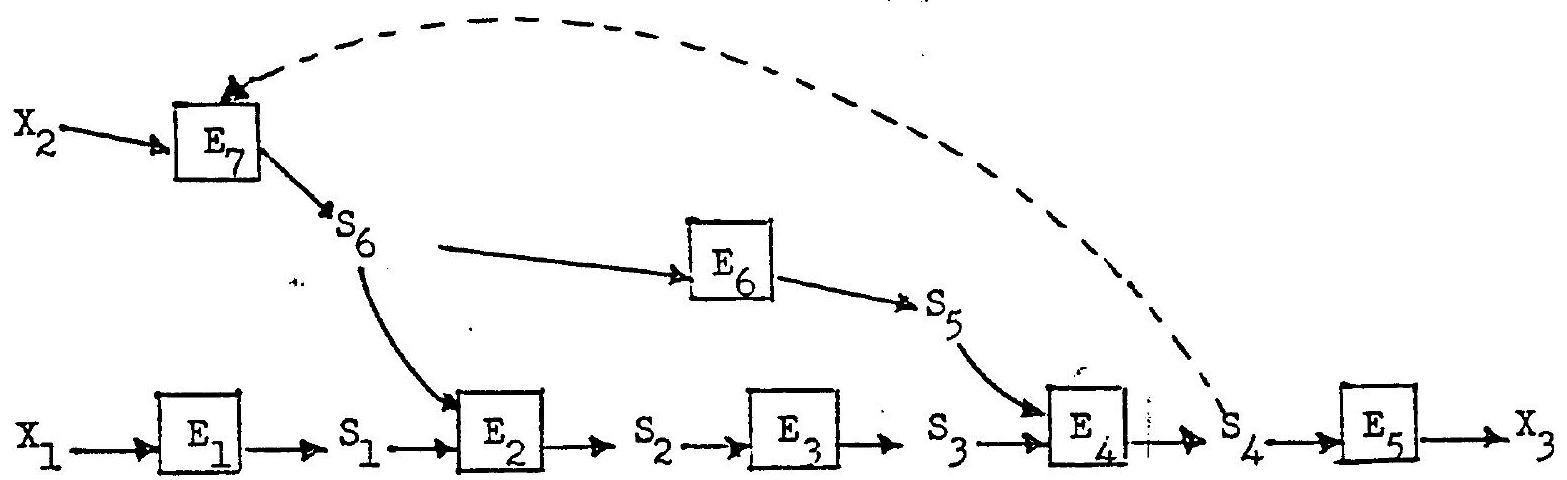
\includegraphics[max width=0.9\textwidth]{2023_01_30_a974a42f7b7381f3f940g-155}
\end{center}

Suppose further that the observed fractional responses of the common flux $F$ and pools $S_{1}, \cdots, S_{6}$ to unknown but small modulation in $\mathrm{X}_{1}, \mathrm{X}_{2}$ and $\mathrm{X}_{3}$ is given in the table below.

\vspace{6pt}
\centerline{OBSERVED RESPONSE IN:}
\vspace{6pt}

MODULATE $\left\{\begin{array}{c|ccccccc|}\hline & \mathrm{F} & \mathrm{S}_{1} & \mathrm{S}_{2} & \mathrm{S}_{3} & \mathrm{S}_{4} & \mathrm{S}_{5} & \mathrm{S}_{6} \\ \hline \mathrm{X}_{2} & 0.2 & 1.8 & 1.2 & 1.0 & 0.2 & -0.6 & -0.4 \\ \hline \mathrm{X}_{2} & 0.2 & -0.2 & 0.2 & 0 & 0.2 & 0.4 & 0.6 \\ \hline \mathrm{X}_{3} & 0.15 & 0.15 & -0.6 & 0.75 & 0.15 & -0.45 & -0.3 \\ \hline\end{array}\right.$

\medskip
Using these data with the method just explained we can apply equations of type (3.52) to find that, for example, the elasticities of $\mathrm{E}_{2}$ with respect to $S_{1}, S_{6}$ and $S_{2}$ are $1, 1,-1$ respectively. For enzymes such as $E_{3}$ which have only two elasticities any two out of the three possible equations will be equivalent. Calculating all the elasticities in this way and using them to construct the sensitivity matrix we obtain

\begin{center}
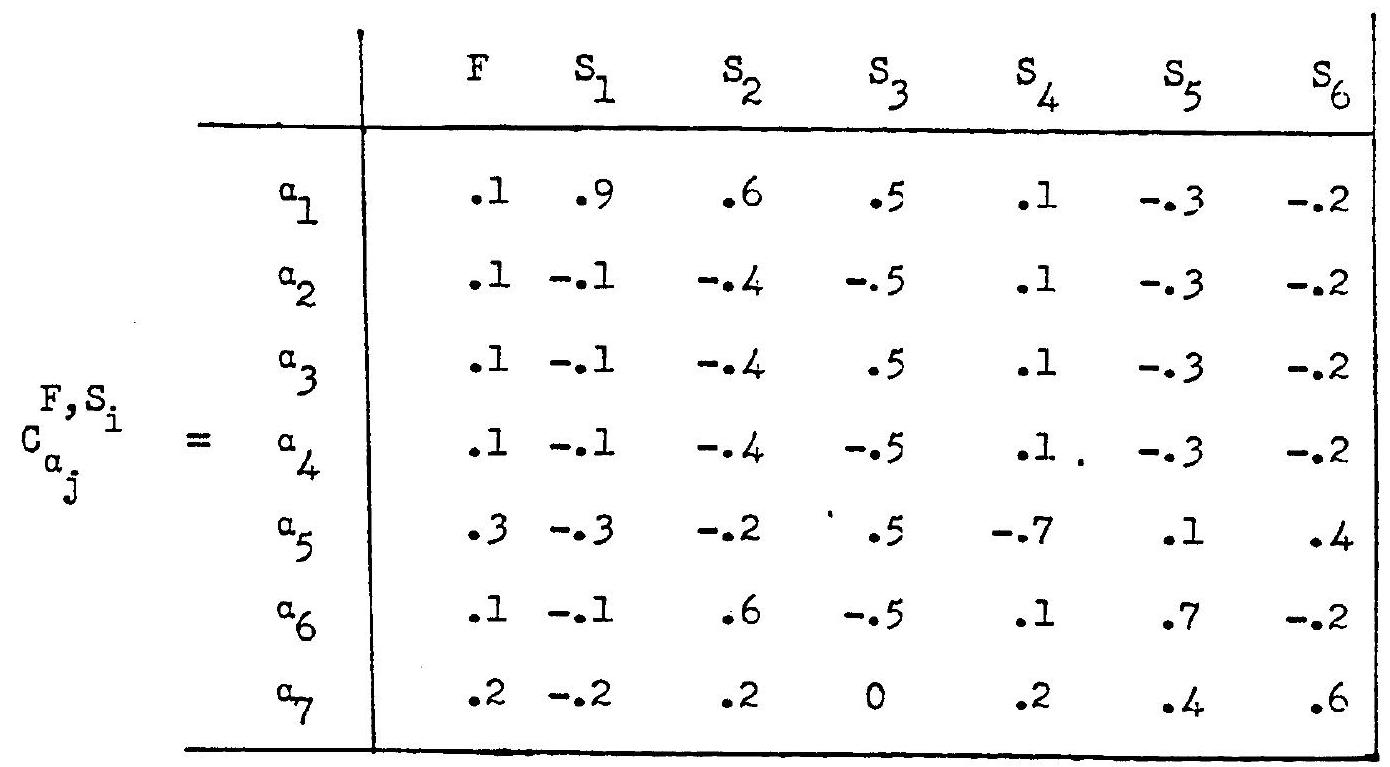
\includegraphics[max width=0.9\textwidth]{2023_01_30_a974a42f7b7381f3f940g-156}
\end{center}

This result will be true even if the different pools have different `extractibilities' and it involves no knowledge of equilibrium ratios or other absolute kinetic quantities. In addition it has been obtained using data from only, three modulation experiments which themselves involve no manipulation of genetic parameters or even knowledge of the size of the modulations.

When performing the necessary modulation experiments it may happen that an X modulation which produces measurable but small responses around one enzyme will produce large changes around another. In such cases it is quite in order to obtain data for the second enzyme using a lower level of modulation, since the equations (3.52) are entirely `Local' in nature. For more complex systems having several independent fluxes it will be necessary to use the observed fractional flux responses to calculate also the stoichiometric elasticities by means of equations similar to (3.52). Inspection of the structure diagram will indicate which of these stoichiometric elasticities will be non zero for each of the enzymes. The sensitivity matrix for such a system can then be found using the additional relations (3.33) which involve the stoichiometric elasticities, the arginine cycle example given earlier illustrates this.

We wish now to consider briefly what problems might arise if the given response data were interpreted on the basis of \underline{wrong} assumptions about the stricture. In particular it is of interest to know whether such errors can be detected by analysis of the given data alone or whether further data becomes necessary.

The diagrams below show a simple example of such a situation Indicating, on the left, the `true' structure, the experimental data on which it is based and the sensitivity matrix which results. On the right of the diagram the situation is shown where the existence of the feedback inhibition is, wrongly, not taken into account and the sensitivity matrix is computed on the basis of only the $X_{1}, X_{2}$ modulation data.

%\begin{center}
%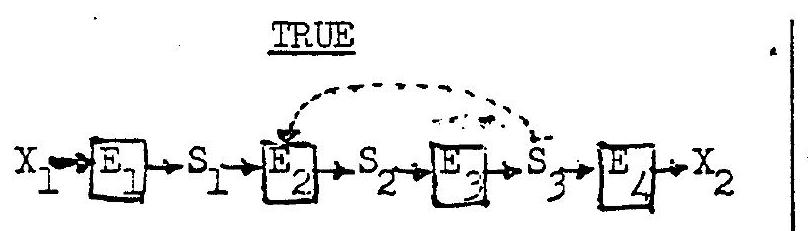
\includegraphics[max width=\textwidth]{2023_01_30_a974a42f7b7381f3f940g-158}
%\end{center}

\begin{center}
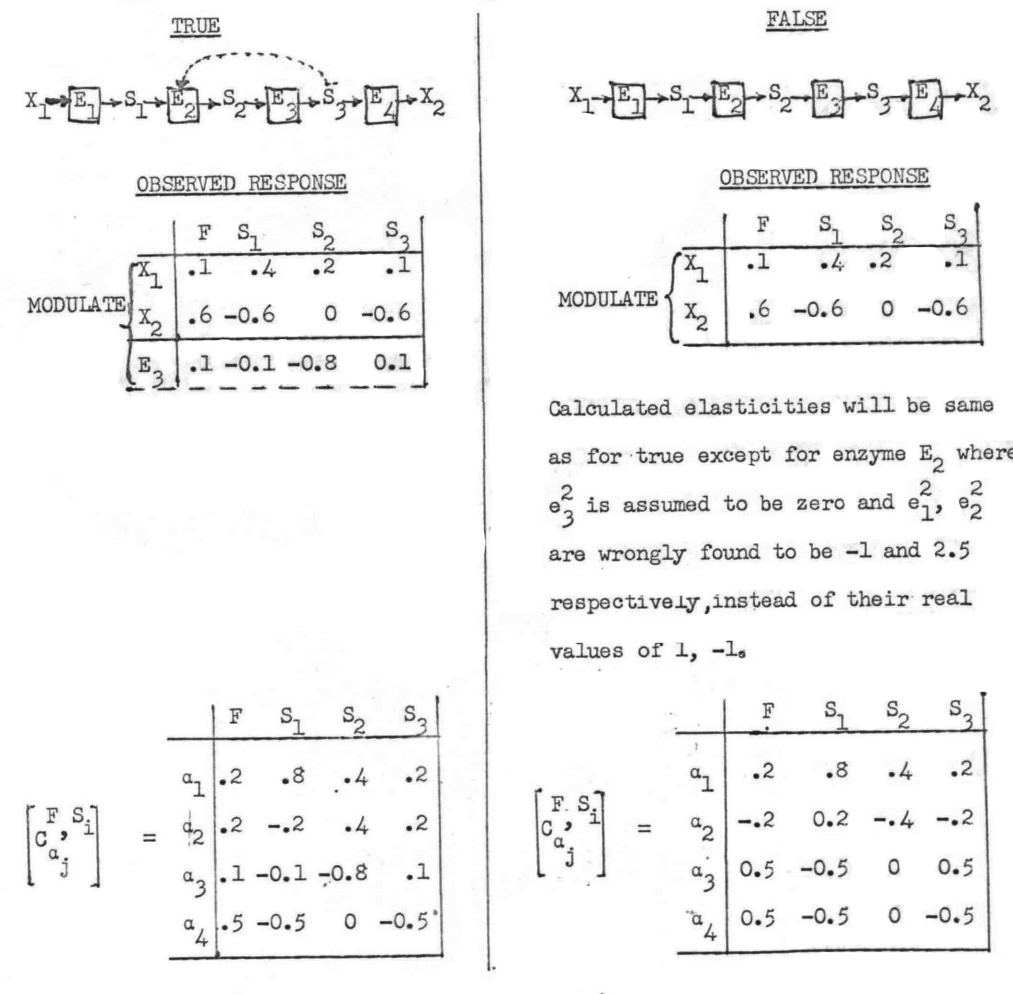
\includegraphics[max width=\textwidth]{figure3_observed.png}
\end{center}

%Calculated elasticities will be sa as for true except for enzyme $\mathrm{E}_{2} \mathrm{w}$ $\varepsilon_{3}^{2}$ is assumed to be zero and $\varepsilon_{1}^{2}, e$ are wrongly found to be $-1$ and $2.5$ respectively, instead of their real values of $1,-1$.

Inspection of the above reveals that the matrix deduced from the limited data and based upon false assumption about structure is nevertheless completely compatible with the given data. By this is meant that the 1st and 4th rows of the matrix are indeed proportional to the observed $X_1, X_2$ response vectors. However the unusual elasticities found for enzyme $\mathrm{E}_2$, which in this example are the reverse of the normal pattern of substrate activation and product inhibition, should warn the investigator that his assumptions about structure may be false. Only when further investigation has revealed the true stricture and suitable extra data has been obtained, by modulating $E_3$, can the correct matrix be found. Further consideration shows that whenever such `loops' are in fact present then the discovery of the true matrix will always involve the use of a revertant affecting an enzyme within the loop.

\section{Modulation to determine elasticities and coefficients}

{\bf Use of genetic modulation to determine elasticities and coefficients within a subsystem}

Because of the very large number of pools and enzymes in wry real biological system the experimenter will normally confine himself to observation on only a small part of it, perhaps to the values of pools ana fluxes in a few related pathways. Such a subsystem, A, together with all pools influencing it, $S_{1}, S_{2}$ and $S_{3}$ for example, is indicated below.

\begin{center}
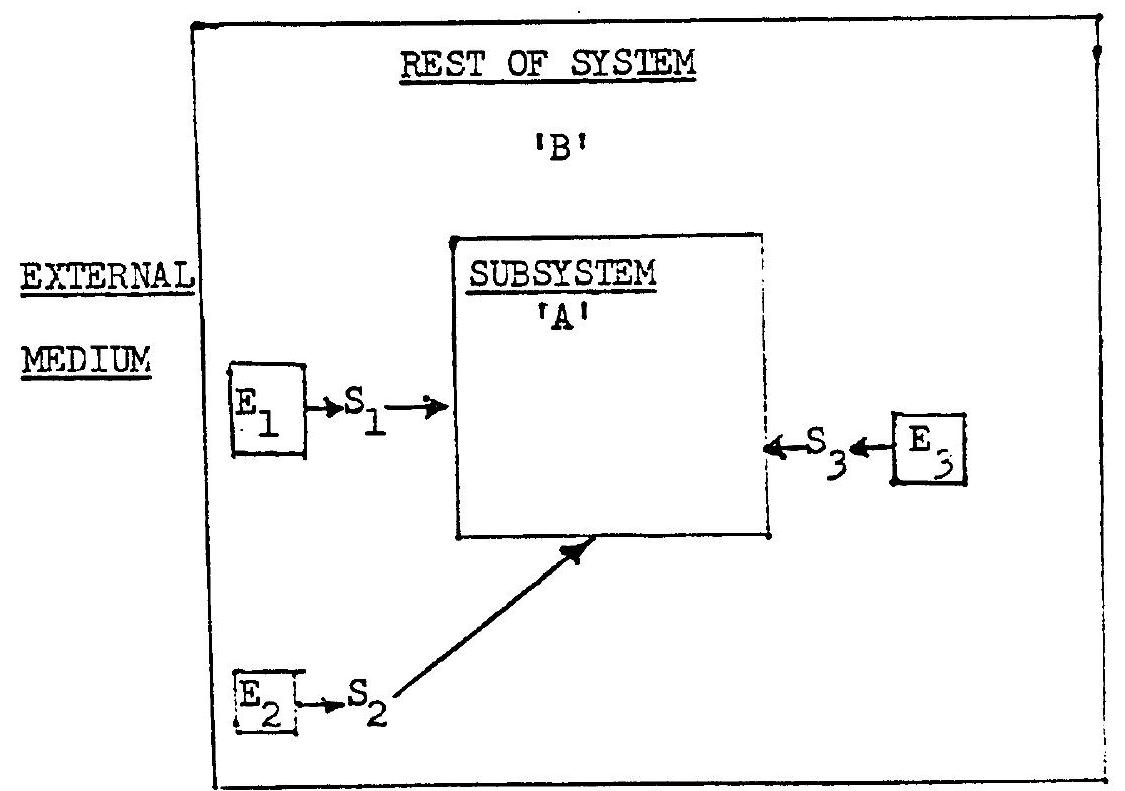
\includegraphics[max width=0.7\textwidth]{2023_01_30_a974a42f7b7381f3f940g-160}
\end{center}

Genetic manipulation in B, possibly via the substitution of altered enzymes at $\mathrm{E}_{1}, \mathrm{E}_{2}$ or $\mathrm{E}_{3}$, can produce several independent response vectors for the pools and fluxes within and around A. How many such modulations will be actually required to estimate the elasticities of all enzymes in A depends on the structure of A. In particular if A contains loops or other complications it may in audition be necessary to use further substitutions actually within the subsystem `$A$'. Once these elasticities have been determined we can write as many 'pool'  relations of type (3.26) connecting the coefficients with respect to blocks inside $A$ as there are pools inside $A$.

However, further information will still be required since the number of blocks in A must always, exceed the number of pools by at least one. This information can be provided by direct measurement, using the methods described earlier, of one or more suitably chosen coefficients within A which can then be used together with the `pool' relations for A to determine the remaining coefficients. This approach involves the labour associated with the necessary `directly measured' coefficients but is much less laborious than direct measurement of all coefficients in A.

Alternatively if certain overall assumptions can be made about the structure of $B$ this difficulty can be completely avoided. The difference between these two methods will be made clear in the following example.

\section{Determination of $C^{F_{1} S_{i}}_{\alpha_J}$ for a system}

\subsection*{a) Making limited use of internal modulation data.}

Suppose that the complete metabolic system is shown below and let the subsystem of interest and the rest of the system be `A' and `B' respectively:

\begin{center}
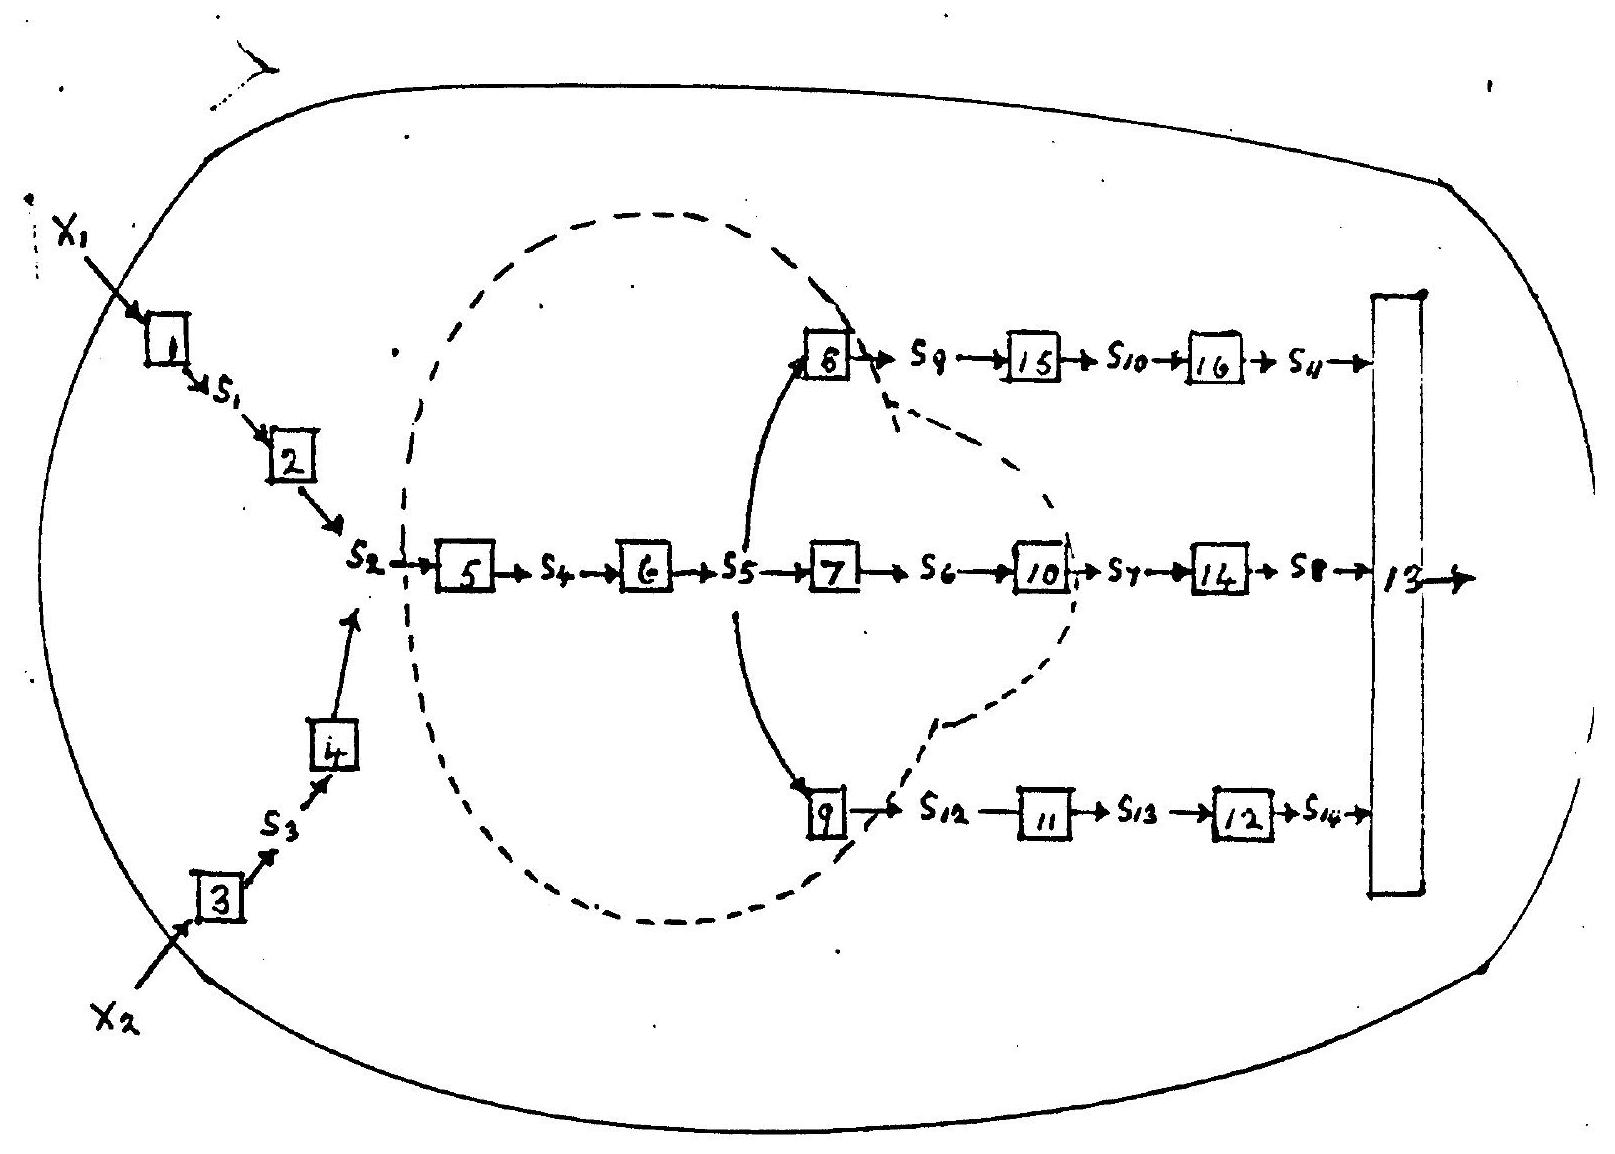
\includegraphics[max width=0.8\textwidth]{2023_01_30_a974a42f7b7381f3f940g-162}
\end{center}

If no assumptions are made about the structure of $B$ then we may proceed as follows. Since no enzyme inside A has more than two elasticities, substitution of, say, $\mathrm{E}_{2}$ and $\mathrm{E}_{14}$ in $\mathrm{B}$ will provide sufficient pool and flux modulations to determine elasticities within A. These elasticities can then be used with pool relation for $S_{4}, S_{5}$ and $S_{6}$ to write down the equations connecting the six block coefficients within A. If now absolute coefficients for $E_{7}, E_{8}$ and $E_{9}$ are determined directly and the others found from them then the process will be complete.

\subsection*{b) Using only internal modulation data.}

The alternative process, which avoids the laborious direct determination of coefficients within A, involves knowledge of the structure of $B$ and is as follows. From the point of view of subsystem $A$ the details of $B$ need not be known except that it can be regarded as made up of two lumped parts $\mathrm{B}_1$ and $\mathrm{B}_2$ as shown below.

\begin{center}
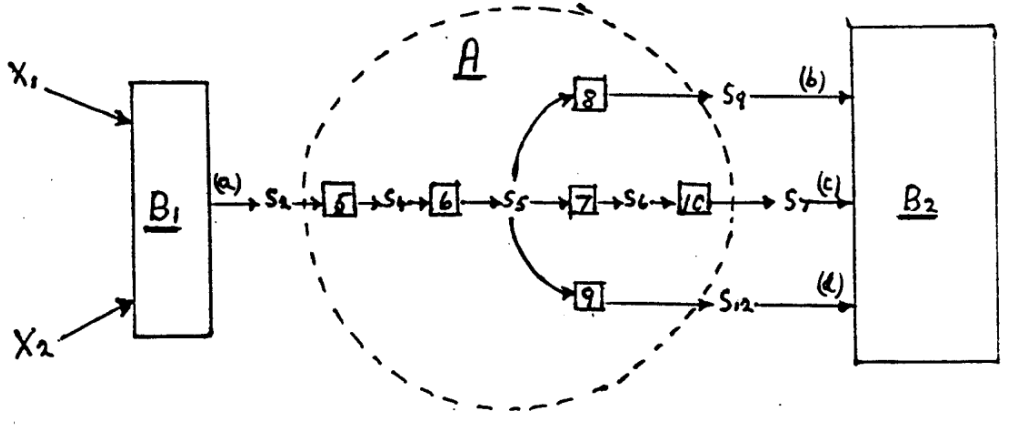
\includegraphics[max width=0.9\textwidth]{figure3_bInternal.png}%2023_01_30_a974a42f7b7381f3f940g-163}
\end{center}

As before all elasticities within A can be found by substitution in $B_{1}$ and $B_{2}$ and in addition the effective elasticity `a' of the subsystem $B_{1}$ with respect to $S_{2}$. Finally the same substitution in $B_{1}$ together with two more made within $A$, say at $E_{8}$ and $E_{9}$, will together provide sufficient date to determine the elasticities, $(b, c$ and $d)$ of the lumped block $B_{2}$. From these elasticities and the simplified structure the true absolute coefficients within A may be determined. Thus, provided the structural assumptions are correct, the experimental effort is just that of determining pool and flux responses for the subsystem A for four substitutions about which nothing need be known except that their effects be not too large.

This latter approach involves exploiting to the full all structural knowledge of the larger metabolic system which will have been gained by a variety of qualitative methods over many years. It seems to offer the best hope of making a `quantitative' estimate of the relative importance of different transformational steps, or blocks, since it builds effectively on existing qualitative information and involves only a minimum of quantitative data which need not involve any absolute measurements. The difficulties in the method arise mainly from the difficulty in determining with reasonable accuracy the small fractional changes in pools and fluxes which are needed and this will be particularly severe in the case of flux determinations.

\section{Optimal allocation for growth}

At the end of CHI.II it was shown that a fairly general model giving the S.S. of a `complete' growing system was defined by the form% determination of coefficients within A, involves knowledge of the structure of $B$ and is as follows. From the point of view of subsystem $A$ the details of $B$ need not be known except that it can be regarded as made up of two lumped parts $\mathrm{B}_1$ and $\mathrm{B}_2$ as shown below.
%
$$ \sum \lambda_{ij} g_j f_j(\olsi{S})-\frac{g_0}{\sum g_j} \cdot g_p \cdot k \cdot f_p(\olsi{S}) \cdot \olsi{S}_i=0 $$
%
The growth rate, $G$, being given by the measure:
%
$$G=\dfrac{g_{p} f_{p}(\olsi{S})}{\sum_{g_j}}. $$
%
We now wish to consider, for a system where the $g^{\prime}s$ are given as parameters, what configuration of the allocation vector $\left[g_{1}, g_{2}, \cdots\right]$ will maximise $t$ growth rate.

Provided the allocation to structure is small compared with that to active protein $\frac{g_{0}}{\Sigma g_{j}}$ will be small and it is possible to treat the problem in a simple way. Thus under these circumstances the problem becomes identical to one where the $\mathrm{E}_{j}$ are given as parameters and the S.S. is defined by
%
$$
\sum \lambda_{ij} E_{j} f_{j}(\olsi{S}) = 0
$$
%
The aim being to maximise the growth rate, $G=\frac{E_{p} f_{p}(\olsi{S})}{\sum E_j} = \frac{F_P}{\sum E_j}$ by adjusting the different enzymes. This can be done by adjusting only the \underline{ratio} of the enzymes whilst keeping their sum constant, since it is only the ratio of the enzymes which affects G. When the optimal allocation exists a small change in the ratio of any two enzymes such that the sum remains constant will have no effect on the flux to protein $F_{p}$ Thus if an amount $\Delta \mathrm{E}$ is transferred from $E_{k}$ to $E_{j}$ around this optimum condition we must have
%
$$
\frac{\Delta F_P}{F_P} = 0 = C_{\alpha_{j}}^{F_P} \frac{\Delta E}{E_{j}} - C_{\alpha_{k}}^{F_P} \cdot \frac{\Delta E}{E_{k}}
$$
%
So that, when optimal allocation exists, we have for any two enzymes $j$ and $k$
%
\begin{equation}
E_{j} : E_{k} = C_{\alpha_{j}}^{F_P} : C_{\alpha_{k}}^{F_P}
\label{eqn:353}
\end{equation}

What this pattern of coefficients and enzyme concentrations actually turns out to be will of course depend on the details of the separate enzymic proteins and the network in which they are embedded. If one of them, for example, has a very low turnover number it will, even at its optimal allocation, require a large amount of protein and have a large coefficient. The following example will make this clear.

\section{Straight chain of linear enzymes}

Consider the chain of enzymes shown below, where $\mathrm{X}$ is the initial substrate and the final reaction is irreversible. The activity, of the separate enzymes is now given as the product, $E_{i} \cdot t_{i}$, of enzyme quanti ty and turnover number

\begin{center}
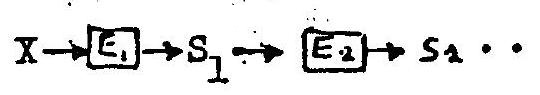
\includegraphics[max width=\textwidth]{2023_01_30_a974a42f7b7381f3f940g-166}
\end{center}

Provided the pools are scaled so that all equilibrium constants are effectively unity the relations (1.18) and (1.19) of CH.I giving the flux and the $C_{\alpha_{1}}^{F}$ can be written as follows. Thus
%
\begin{equation}
F=\frac{X}{\sum \frac{1}{V_{i}}} = \frac{X}{\sum \frac{1}{E_i \cdot t_{i}}}
\label{eqn:354}
\end{equation}
%
and
%
\begin{equation}
C_{\alpha_{i}}^{F} = a \cdot \frac{1}{V_{i}} = a \cdot \frac{1}{E_{i} \cdot {t_i}}
\label{eqn:355}
\end{equation}
%
Where $a$ is the same constant for all enzymes.

We can now apply the relation (3.53) in order to discover the optimal allocation of enzymes which will maximise $F$ for a given total enzyme $E_{T}$ and ensure the maximum growth rate.

Thus $(3.53)$ can be written as
%
$$
E_{i}=b \cdot C_{\alpha_{1}}^{F} \text { where } b \text { is the same constant for all enzymes }
$$
%
and combined with the expression (3.55) for the coefficients this gives
%
$$
E_{i}=b_{\cdot} C_{\alpha_{i}}^{F} = a \cdot b \cdot \frac{1}{E_{i} t_{i}}
$$
%
or
%
$$
E_{i} \propto \frac{1}{\sqrt{t_{i}}}
$$
%
Hence we have that the optimal allocation of enzymes in the chain is such that
%
\begin{equation}
E_{1}: E_{2}: E_{3}: \cdots=\frac{1}{\sqrt{t_{1}}}: \frac{1}{\sqrt{t_{2}}}: \frac{1}{\sqrt{t_{3}}}:
\label{eqn:356}
\end{equation}
%
To find the corresponding maximum growth rate we must use this enzyme ratio in (3.54) to give $F_{\max}$ for a given $E_{T}$ Thus from (3.56) we have
%
$$
E_{i} = E_{T} \frac{\frac{1}{\sqrt{t_{i}}}}{\sum \frac{1}{\sqrt{t_{i}}}}
$$
%
and $\dfrac{1}{E_{i} \cdot t_{i}} = \dfrac{\sum \dfrac{1}{\sqrt{t_{i}}}}{E_{T} \sqrt{t_{i}}}$. Putting this into (3.54) we now get
%
$$
F_{\max} = \frac{X_{\cdot} E_{T}}{\left(\sum \frac{1}{t_{i}}\right)^{2}}
$$
%
So that the maximum growth rate is
%
\begin{equation}
\mathrm{G}_{\max } = \frac{F_{\max}}{E_{T}} = \frac{X}{\left(\sum \frac{1}{\sqrt{t_{i}}}\right)^{2}}
\label{eqn:357}
\end{equation}
%
In particular suppose that the chain consisted of three enzymes having turnover numbers of 1, 4 and 9 respectively and that $X=1$ and $E_{T}=9$. If the enzymes are allocated equally the growth rate is given by calculating $\frac{F}{E_{T}}$ using $(3.54)$ giving
%
$$
G=\frac{1}{9} \cdot \frac{1}{\frac{1}{3}+\frac{1}{3 \times 4}+\frac{1}{3 \times 9}} \quad=0.25
$$
%
on the other hand $G_{\max}$ for optimal allocation is given by (3.57) as
%
$$
G_{\max } \bumpeq \frac{1}{\left(1+\frac{1}{2}+\frac{1}{3}\right)^{2}} = 0.3
$$
%
In this case optimal allocation of the enzyme has only improved the growth rate by approximately $20 \%$ from that obtained with an equal allocation.

\section{Optimal solution given alternative food sources}

Consider the three linear enzymes shown below.

\begin{center}
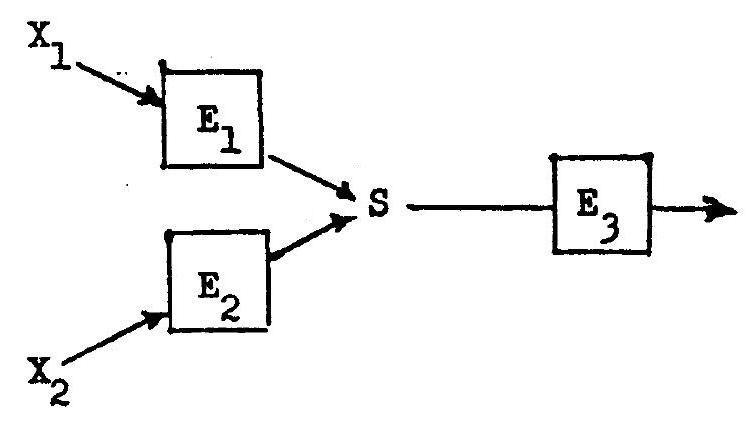
\includegraphics[max width=0.5\textwidth]{2023_01_30_a974a42f7b7381f3f940g-168}
\end{center}

In this case, if we consider $\mathrm{F}_{3}$ as the flux to protein, the problem is to find the best allocation between $\mathrm{E}_{1}, \mathrm{E}_{2}$ and $\mathrm{E}_{3}$ It can be shown by a simple argument that the maximum must be one or other of the solutions in which either $\mathrm{E}_{1}$ or $\mathrm{E}_{2}$ is zero. Using the previous example this gives the maximum as being the greeter of the two expressions
%
$$
\frac{X_{1}}{\left(\frac{1}{t_{1}}+\frac{1}{t_{3}}\right)^{2}} \quad\text{ and }\quad \frac{X_{2}}{\left(\frac{1}{t_{2}}+\frac{1}{t_{3}}\right)^{2}}
$$
%
This means that, depending on the ratio of $X_{1}/X_{2}$, the optimal organism of this type will choose to feed exclusively on one or other of the alternative nutrients but never on both.

\subsection*{Role of regulation}

It seems clear that for organisms such as E.coli where growth rate is of great selective value, an important role for the regulatory loops found may be to adjust the enzyme allocation so that it approximates to optimal over a variety of environmental situations.

In computer studies it will be of interest to introduce suitable regulatory functions for the $g_{i}$, which can respond to both $X$ and $S$ values, and to compare the allocations achieved by such systems with the computed optimal allocations over a range of environmental situations. Such studies could give us some quantitative idea of the value, from the point of view of maintaining a high growth rate, of the various regulatory mechanisms found. 